\newcommand{\homedir}{/home/bscholtz/workspace/workspace-latex/2016-Design-Project/LATEX/}

%######################Preamble######################
\input{"\homedir preamble.tex"}

\newcommand{\coursecode}{EEE4036A}
\newcommand{\assignment}{Parking System Design Project\\Team 14}
\newcommand{\lecturer}{Riana Geschke}

\pagestyle{fancy}
\fancyhf{}
\rhead{Design Project}
\lhead{Team 14}
\cfoot{\thepage}

\begin{document}

%######################Title Page######################
\begin{titlepage} 

\includegraphics[width = 17cm]{images/uctbanner.png} \\

\begin{center}
\begin{LARGE}
Faculty of Engineering and the Built Environment \\
Department of Electrical Engineering \\
\end{LARGE}
\end{center}

\begin{center}  
\begin{Huge}
\textbf{\coursecode}\\
\bigskip
\bigskip
\hrule
\assignment \\
\end{Huge}

\vspace*{\fill}

\hrule
\begin{center}
\textbf{Benjamin Scholtz (SCHBEN011)\\
Jarushen Govender (GVNJAR002)\\
Isaac Lebogang Khobo (KHBISA001)\\
Nasko Stavrev (STVATA001)\\}
4$^{th}$ year BSc. (Eng.) Electrical Engineering Department\\
Lecturer: \lecturer \\
\today
\end{center}
\bigskip
\hrule

\end{center}
\end{titlepage}

%######################Contents######################

\newpage
%\section*{Contents}
%\addcontentsline{toc}{section}{Contents}  
\tableofcontents

%######################Plagiarism Dec.######################
\input{"\homedir plagiarism-declaration.tex"}

%######################Begin Content######################
\newcommand{\lsec}[1]{\normalsize{\textbf{#1}}\\}

\newpage

\section{TASK CLARIFICATION}
\subsection{Background}
UCT Upper campus has a number of parking areas for staff, students and visitors using cars to travel to campus. There are red, yellow, blue/unmarked bays on campus. In addition there are disabled and 
visitor parking bays on campus. These categories are assigned the highest priority. 

For every user, a parking category is assigned, and an associated annual fee is charged.  The purchase of a parking disk allows the staff member/student/visitor to search for a parking spot in the designated category on campus, but it is not guaranteed that one will be available, since parking bays are oversold. When arriving on campus, a driver of a car may spend some time searching for an available spot in the required category. Parking disks are generally linked to a person and only valid for the specific vehicle for which the disk has been purchased, except for student lift clubs.

The Traffic  Department  on  Upper  Campus  administrates  and  manages  all  aspects  related  to  parking  of vehicles.\cite{assignment}

In the figure below a survey of UCT students was completed to determine of those students who owned a blue parking disk, how many of them would park illegally in the case of there being no more blue parking bays on upper campus. The results clearly indicate that illegal parking is a problem with the current UCT parking system.

\begin{figure}[H]
\begin{center}
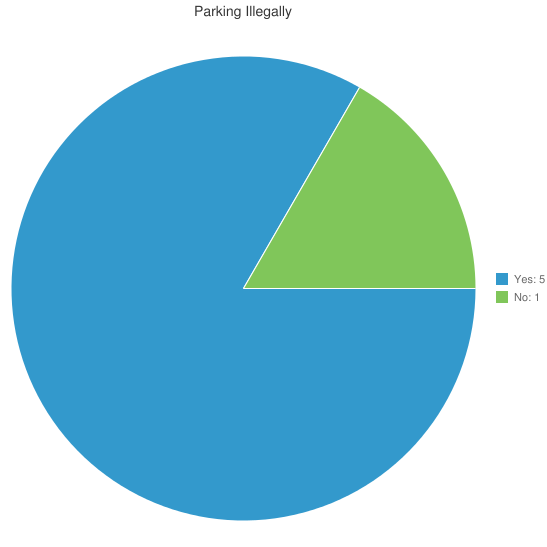
\includegraphics[scale=0.55,clip]{data/chart.png}
\caption{Illegal parking on UCT upper campus.}
\end{center}
\end{figure}
 
\subsection{Problem Statement}
For  a  driver  entering  Upper  Campus  in  a  car,  it  is  not immediately  apparent  where  there  are  parking bays available.  This is a particular problem during peak times when a large number of cars arrive on campus, looking for parking at the same time. The second problem that exists is that these users then choose to park illegally if a parking bay can not be found (as shown in the figure above). The design assignment is to solve this problem using the electrical engineering skills of each of the team members in our group.\cite{assignment}

The design assignment is:

\begin{itemize}
\item To provide information in an easily accessible format, to each driver of a car immediately on arrival on campus, on where all the vacant parking bays on campus are. This must be for the specific category of parking for this user.

\item To determine whether a vehicle is parked on a bay not designated for this user, for example a yellow disk holder parks on a red bay, or a visitor parks on a disabled parking bay, and make this available to the traffic department in real time.

\item To  allow electronic reconfiguration  of  traffic  bay allocations  on  special  occasions, for example during the summer school period, when there are many visitors requiring parking on campus.

\item To monitor and log the use of parking bays and the percentage of occupation of each parking area and make this available to the traffic department, for the purpose of planning.\cite{assignment}
\end{itemize}



\newpage
\section{CONTEXT OF DESIGN}
\subsection{Macroeconomic Factors}
\subsubsection{Technical} 
In South Africa there are a number of technical concerns to deal with regarding the production of electronic systems. The PCB design standards in South Africa are not of as high a standard as in certain overseas production houses and may have longer production times. The system might take a specialized skill set to maintain and repair the system components. Both of these factors need to be dealt with to achieve a balance between quality, production time and capital outlay for the system.

\subsubsection{Economic}
The current South African economy lends itself to local production of goods using cheaper local labour. The problem with local production is that it is still expensive to import the components and materials needed for the production - this can be justified considering that there may be a possibility to export any products developed as the economy lends itself to the export of goods to foreign markets. 

\subsubsection{Ethical}
A few ethical issues arise as soon as people or vehicles are equipped with electronics capable of tracking or logging movement and actions. Users will have to be made aware of the risks or lack there of. Legal advice will need to be used to draw up user agreements for the system. The ethics of tracking users will need to be considered and systems put in place to ensure users can not be tracked off campus, and that the data collected on campus is securely encrypted or stored.

\newpage
\subsection{Microeconomic Factors}
\lsec{UCT Parking Cash Flow}
To calculate the upper campus UCT parking cash flow in the table below, a few assumptions were made. Approximately 2.8 parking discs are allocated per bay. Assuming this is true of all parking bay categories, this results in a total cash flow of R13.6 million per year. Assuming that 20\% of this cash flow is used for maintenance, and the other 20\% for parking staff salaries, we are left with R8.16 million for the project, with possible external funding if necessary.

The following table shows the number of different privilege level parking spots  and what the user pay for those slots, as well as how many users are allocated to those spots in order to calculate the cash flow acquired from the user yearly disc payments.

\begin{table}[H]
\centering
\caption{Upper Campus UCT Parking Cash Flow}
\label{cash-flow}
\begin{tabular}{lllll}
                         & \textbf{Parking Bays} & \textbf{Allocated Bays} & \textbf{Disc Price (R)} & \textbf{Cash Flow (R)} \\
\textbf{Red}                      & 808                   & 2262.4                  & 1524                & 3447897.6          \\
\textbf{Yellow}          & 1046                  & 2928.8                  & 960                 & 2811648            \\
\textbf{Student}         & 2757                  & 7719.6                  & 960                 & 7410816            \\
\textbf{Total Bays}      & 4611                  & 12910.8                 &                     &                    \\
\textbf{}                &                       &                         &                     &                    \\
\textbf{Discs/bay}       & 2.8                   &                         &                     &                    \\
\textbf{Total Cash Flow} & R13670361.6            &                         &                     &                   
\end{tabular}
\end{table}

From the table above and with with calculated R8.16 million available for research and development, the project capital expenditure should be below R5 million - this leaves enough capital for unforeseen expenses, either from oversight or incurred risk.

\lsec{Social Behaviour}
UCT parking system users are currently forced to take illegal action when locating and using parking bays due to a lack of parking bays available. The new system will have to address these issues and the mindset of the parking system users will have to change to accept the new system that will introduce more red tape and make it harder for them to get away with parking illegally. This could be addressed by having a parking system that adjusts to the regularity at which a user parks and charging them accordingly - this will motivate users, even if they are in possession of a disk, to find other means of transport on certain days, thus reducing the parking system load.

\newpage
\section{DESIGN SPECIFICATION}
\subsection{Scope}
This specification covers the analysis, design, production timeline and considerations, and lifecycle of the upgraded UCT parking system. The specification is for a parking system on upper campus to be used primarily in allocated parking zones rather than dispersed parking bays. The parking system specifications aim to meet the requirements introduced in the client problem statement.

\subsection{Applicable Documents}
The following documents are applicable to the project and are of importance to the ultimate specifications of the project:
\begin{itemize}
\item Group Allocation
\item Group Project Assignment
\item Design Notes
\end{itemize}

\subsection{Characteristics}
\subsubsection{Functional Characteristics}
\lsec{Function 1: User interface} 
Information must be available in an easily accessible format to indicate to drivers where legal parking bays are located.

\lsec{Function 2: Vehicle location}
Real time location and classification of vehicles in UCT parking areas based on user parking privileges. 

\lsec{Function 3: System back-end}
Traffic department should be able to access data about vehicles and users on a database as well as reconfigure traffic bay allocations. The use of parking bays should be monitored and logged to be processed to show percentage occupation of parking area and get historical data.

\lsec{Interface Characteristics} 
Function 1, 2 and 3 should be linked with a wireless communication method.

\newpage
\subsubsection{Quality Assurance}
\lsec{Standards and Codes}
The design must meet the following standards and codes:
\begin{itemize}
\item IEEE Standards.
\item SABS Standards.
\item ICASA RF Regulations.
\item RF PCB Design Standards.
\end{itemize}

\lsec{Methods of Testing}
The design should be tested using the following method:
\begin{enumerate}
\item Periodic random parking bay testing.
\item HIL system testing.
\item Brute force user and operator interface testing.
\item Long term power system testing.
\item RF propagation testing.
\end{enumerate}

\lsec{Reliability Issues}

Reliability issues will arise in the following forms:

\begin{itemize}
\item Component quality standards.
\item Supplier reliability (especially for importing).
\item User familiarity with the system.
\item Unknown environment variables (RF signal propagation, mechanical obstructions etc.)
\item Unknown user variables (User behaviour etc.)
\end{itemize}

\newpage
\subsubsection{Timescale}
\lsec{Design Schedule}
The embodiment design should be completed within the given period of just under two months, in time for hand in after the first UCT term.

\lsec{Development Schedule}
Thereafter the final design should be developed and tested within a period of 4 months; and certified with the relevant organisations within a period of 2 months.

\lsec{Production Schedule}
The final design should be prototyped over a period of 1 month and then any necessary changes completed within 1 month thereafter - a final product will be sent for production over the course of 1 month. The necessary traffic department staff training and student/user familiarisation will be completed during the production time period over a period of 2 months.

\lsec{Delivery Schedule}
The complete system will be installed and in use over the period of 1 month. 

\begin{figure}[H]
 \begin{ganttchart}[x unit=10mm, y unit chart=0.8cm]{1}{12}
\gantttitle{\textbf{Year of Implementation (months)}}{12} \\
\gantttitlelist{1,...,12}{1} \\
\ganttgroup{Design Schedule}{1}{2} \\
\ganttbar[bar/.append style={fill=yellow}]{Embodiment Design}{1}{2} \\
\ganttgroup{Development Schedule}{3}{8} \\
\ganttbar[bar/.append style={fill=blue}]{Final Design}{3}{6} \\
\ganttbar{Certification}{7}{8} \\
\ganttgroup{Production Schedule}{9}{11} \\
\ganttbar[bar/.append style={fill=blue}]{Prototype and Testing}{9}{9} \\
\ganttbar{Final Changes}{10}{10} \\
\ganttbar[bar/.append style={fill=blue}]{Final Production}{11}{11} \\
\ganttbar[bar/.append style={fill=red}]{Training and Familiarisation}{9}{10} \\
\ganttgroup{Delivery Schedule}{12}{12} \\
\ganttbar[bar/.append style={fill=red}]{Installation}{12}{12} \\
%\ganttmilestone{Milestone}{11} \ganttnewline

\ganttlink{elem1}{elem3}
\ganttlink{elem3}{elem4}
\ganttlink{elem4}{elem6}
\ganttlink{elem6}{elem7}
\ganttlink{elem7}{elem8}
\ganttlink{elem2}{elem9}
\ganttlink{elem8}{elem11}
\end{ganttchart}
\caption{Project Gantt Chart.}
\end{figure}

\subsubsection{Economic Factors}
\lsec{Market Analysis}
The users of the system will be predominantly students and a small number of staff who may have limited funding for parking disks. The cost of the disks need to be kept at the same price as outlined in the Microeconomic Factors, while adding the advanced functionality needed to meet the design specifications. On questioning users, they responded that they would not be willing to pay more for this advanced functionality - with some saying they still believe the costs for parking on campus are too high considering the lack of available parking on most days. The new parking system should address the above issues.

\lsec{Design Costs}
The design costs will be kept to a minimum by using UCT Electrical Engineering students to complete the design as a part of their EEE4036A design course.

\lsec{Development, Manufacturing, Distribution Costs}
The main costs incurred will be in contracted manufacturing and distribution. 

The following companies will be contracted to:
\begin{enumerate}
\item Zytek will be used for the manufacturing and assembly of the PCBs.
\item Skeg product development will be used for the tag and beacons casing production using injection mould methods.
\item Electronic components will be imported from Mouser predominantly. 
\end{enumerate}

The costs of development, manufacturing and distribution through the above sources should be kept to a unit cost value of less than R400 per tag. This ensures the cost of a disc will cover the cost of production of the tag, assuming  the allocation of funds as outlined in the Microeconomic Factors, with 60\% being left for hardware and software costs.

\subsubsection{Ergonomic Factors}
\textit{\textbf{Device definition:} in the following sections a device refers to whatever user interface and necessary user interactions, whether with software or hardware, are required for the parking system.}

\lsec{User needs}
The user should be able to easily use the interface, whether internal (cellphone app etc.) or external (LED sign board) while driving. The use of the system should not endanger the user by distraction or otherwise. The device should not interfere with the users field of vision.

\lsec{Ergonomics}
The ergonomics of the device should meet the needs of the user. The interface should be easily accessible. The process of installing the device in the car should be self explanatory and not involve a complex process that requires assistance from UCT parking staff.

\newpage
\lsec{Controls}
The controls of the device should meet the needs of the user. The controls should be minimal to avoid complexity and distraction, yes should also allow access to all the functions as set out above in the Functional Characteristics section.

\subsubsection{Life-cycle}
\lsec{Distribution}
Distribution of the device should be on a yearly basis, with user returning the device for maintenance and license renewal.

\lsec{Operation}
The user should be able to install the device easily and have it operate reliably for the period of one year. 

\lsec{Maintenance}
Minimal maintenance (whether for power source or mechanical maintenance or UID configuration) should be required for the device, with a minimum maintenance cycle of one year which is the period a user will be in possession of said device and expect it to operate reliably. Realistically this mean the maintenance cycle should be at least two years for worst case design - this will lessen the risk of a failure during the one year cycle.

\lsec{Disposal}
The device and it's components should, if required to be, be disposed of in a safe manner - this includes batteries and any other harmful substances. The device, after one year of use, should be returned to the parking staff especially during the initial testing phase where the system will be reviewed. The entire system should be operational for a period of at least 15 years. This will ensure that the system makes a return on investment.

\subsection{Acceptance Test Requirements}
\lsec{Function Test Requirements}
The following tests will be put in place to ensure the system meets the functional specifications outlined above before and during the system's operation:

\begin{itemize}
\item \textbf{In-service measurements:} Permanent disk installation (either RFID, Decawave or otherwise) to have a way of testing each parking area is operating correctly without relying on a user reporting the issue.
\item \textbf{Manual inspection:} Weekly inspection during non-peak hours, to randomly test various bays in each section.
\item \textbf{Field trials:} Trial the system in a low-traffic parking area before users are introduced to the system for the first time.
\end{itemize}

\newpage
\section{CONCEPTUAL DESIGN}
\subsection{Design One}
Design One (D1) uses a triangulation system to locate the registered vehicle within the parking area. Each registered vehicle has a tag with a unique ID - this ID has the user data linked to it in a database on the server back-end. The location of each parking space is known, and with the knowledge of where the vehicle is located it can be determined whether the vehicle is legally parked or not. 
  
\subsubsection{System Diagram}
Figure~\ref{fig:soft-overview2} below shows a diagram detailing the overall structure of the system. 

\begin{figure}[H]
\begin{center}
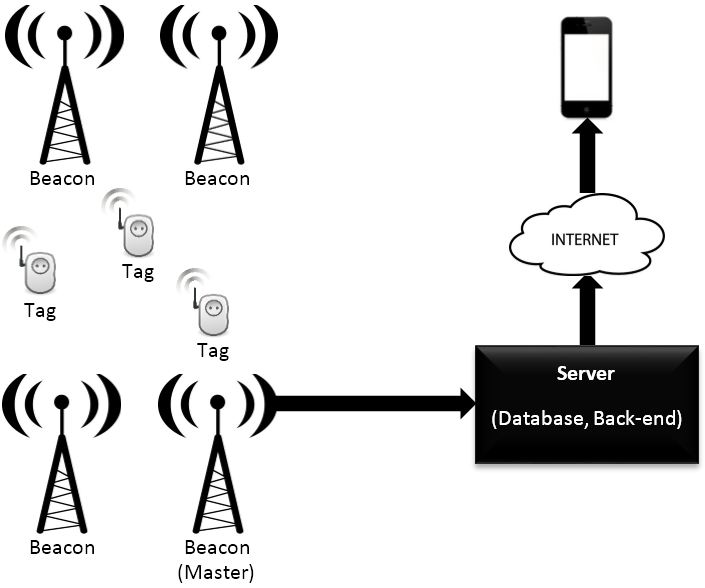
\includegraphics[scale=0.5]{data/software/1.jpg}
\caption{System overview.}
\label{fig:soft-overview2}
\end{center}
\end{figure}

The system uses trilateration to locate the parking system users, relay this information to a server for processing and supply the necessary parking information to the user via a mobile or web interface. This will be further expanded upon in the System Components section.

\subsubsection{System Components}
\lsec{Tags and Beacons}
Due to a triangulation system being used, in every parking area there are at least three beacons - with four being used to try to eliminate signal propagation issues. The tags and beacons make use of a Decawave DW1000 ultra-wideband transceiver chip that is controlled via SPI from a Atmel micro-controller. 

The master beacon sends a signal out to synchronise all the beacons to the same time reference. Each tag sends a signal periodically with the unique user ID, transmit time and battery level which is received by each of the beacons. The beacons all relay time of flight data back to the master beacon which performs a time difference of arrival (TDOA) calculation to determine where the tag is located.\cite{decawave-presentation}

The tags transmit with a period of 5-10 minutes. This reduces power consumption and signal noise level interference with other tags. The tags do not receive data. The tags will be accurate to within 10cm giving more than enough accuracy for the application. The initial conservative battery life estimate is 5 years with proper power management in software. They will be powered with a LiPo battery that will need to be replaced or charged when discharged.

The beacons will use the same circuitry, but with different software running on the Atmel micro-controller. They will be required to both transmit and receive. The beacons will be mounted on poles (both light and installed) distributed across the UCT campus - this will allow the location of vehicles in any area. They will be powered with LiPo batteries which will be charged with solar panels - or wired in cases where this is not practical.

\lsec{Server Back-end}
The server back-end connects with the master beacon via WiFi and receives the tag location, unique ID and battery level for every new vehicle. This is updated on a database every 5-10 minutes. Further calculations and visualizations are performed and stored in the database to send to the end user. The following data will be available for each unique ID:

\begin{itemize}
\item User privileges.
\item Tag location (updated periodically).
\item Tag battery level (updated periodically).
\end{itemize}

\lsec{User Interface}
The user interface will connect with the server back-end to access the database and will relay the following data to the end user via a smart phone application or web application: 
\begin{itemize}
\item Indication of privilege level and violations.
\item Tag battery level.
\item Vehicle location.
\item Location of open parking bays.
\item Recommended parking area.
\item Number of free parking bays in parking area.
\item Traffic heat-map on campus.
\end{itemize}

\newpage
\subsubsection{Requirement Satisfaction\cite{assignment}}
Design One satisfies the design requirements outlined in the Task Clarification section in the following ways:

\begin{itemize}
\item \textbf{To provide information in an easily accessible format, to each driver of a car immediately on arrival on campus, on where all the vacant parking bays on campus are. This must be for the specific category of parking for this user.}\\
Design one satisfies this requirement by not only tracking parked vehicles and where they are, but also the user entering UCT upper campus - this allows the mobile and web GUI system to give user specific directions to the nearest available parking bay.

\item \textbf{To determine whether a vehicle is parked on a bay not designated for this user, for example a yellow disk holder parks on a red bay, or a visitor parks on a disabled parking bay, and make this available to the traffic department in real time.}\\
Each bay will have it's corresponding GPS coordinate in the database. Every car with a disk on campus will be tracked, which means that whenever someone illegally parks the UCT parking department will know. Visitors will have to be allocated visitor discs for the system to work for all cases.

\item \textbf{To allow electronic reconfiguration  of  traffic  bay allocations on special occasions, for example during the summer school period, when there are many visitors requiring parking on campus.}\\
The database will be easily reconfigured to allocate each GPS parking location to a different category of user. Visitors will have to be allocated daily disks, much like they are currently required to do.

\item \textbf{To monitor and log the use of parking bays and the percentage of occupation of each parking area and make this available to the traffic department, for the purpose of planning.}\\
Not only will the design be able monitor and log the use of parking bays and parking areas via the database, the traffic department will be able to see both real-time movement and post-processed heat maps of campus and where cars are located.
\end{itemize}

\subsubsection{Evaluation}
\lsec{Cost} 
The cost of installation of the system will be minimal with the decisions made for costs to be incurred in the distribution of the tags rather than permanent hardware.

\lsec{Implementation}
The implementation of the system will be very efficient, as very little permanent mechanical installations exist. Implementation will involve distribution of the tags and the set up of the server back end. The poles for the beacons will be easily installed. 

\newpage
\lsec{Maintenance}
Maintenance will involve ensuring all tags are working optimally on a yearly basis. The tags are estimated to last on a single 1000mAh LiPo for a period of 3 years. The beacons will most likely need very little maintenance, as they are only subject to weathering and not mechanical impact of vehicles. 

\lsec{Energy Consumption}
As with the tags, the beacons are also very power efficient, with minimal circuitry and a low density per parking area. The tags are an insignificant energy cost. The beacons will run on solar energy, as they can be trickle charged without having to have solar energy every day.

\lsec{Strong/weak Points}
Strong:
\begin{itemize}
\item Low energy usage.
\item Minimal installation effort and costs.
\item Minimal maintenance effort and costs.
\item Low cost system overall.
\item Extensive location information from post-processing.
\end{itemize}

Weak:
\begin{itemize}
\item Relatively expensive tag in high risk environment.
\item Possible RF interference.
\end{itemize}


\subsubsection{Risk Assessment}
\lsec{External Causes} 
Human Interference \textbf{(high risk)}: The users of the system play a big role in the RF performance of the system - the users need to place the tag on the window of the vehicle in order to ensure there is minimal interference from the car body, if the user fails to do this then the system could fail for that user. The tags are relatively expensive, and could be a target for theft.

Weather \textbf{(low risk)}: The intended lifetime of the beacon and tag system is 15 years. Cape Town receives high wind speeds and rainfall - this poses a relatively large risk to the beacons. UV sun damage poses a risk to the housing of the tags, which will be exposed on the windscreen of the vehicle. 

\lsec{Internal Causes}
Failure to recognize long-term design flaws \textbf{(low risk)}: The system is well documented and simple in terms of implementation and maintenance. The risk of long term design flaws lies mainly with the power source of the tags and the RF design of the system. There could also be design issues in the UI that could cause confusion in managing the system.

\newpage
\lsec{Mitigation}
The following steps will be taken to mitigate these risks:

\begin{enumerate}
\item Proper marketing to users and training to staff will be provided prior to the system's installation - this will ensure proper use of the system.
\item Assisted installation of tags for first time users.
\item Proper material engineering design and waterproofing will be implemented to ensure endurance to weathering.
\item Costs will be reduced by eventually manufacturing the product overseas, the tags will also be made low profile to reduce risk of theft.
\item The system will be made modular which means that if one component fails the system continues working. 
\item There will be more than the required number of beacons in each parking area to ensure that if one fails the system continues working and if RF interference comes up, it isn't an issue.
\end{enumerate}

\newpage
\subsection{Design Two}
\subsubsection{System Diagram}
\subsubsection{System Components}
\subsubsection{Requirement Satisfaction}
Design Two satisfies the design requirements outlined in the Task Clarification section in the following ways:

\begin{itemize}
\item \textbf{To provide information in an easily accessible format, to each driver of a car immediately on arrival on campus, on where all the vacant parking bays on campus are. This must be for the specific category of parking for this user.}\\
Description of how it satisfies each requirement...

\item \textbf{To determine whether a vehicle is parked on a bay not designated for this user, for example a yellow disk holder parks on a red bay, or a visitor parks on a disabled parking bay, and make this available to the traffic department in real time.}\\

\item \textbf{To allow electronic reconfiguration  of  traffic  bay allocations on special occasions, for example during the summer school period, when there are many visitors requiring parking on campus.}\\

\item \textbf{To monitor and log the use of parking bays and the percentage of occupation of each parking area and make this available to the traffic department, for the purpose of planning.}\\
\end{itemize}

\subsubsection{Evaluation}
\lsec{Cost} 
(implementation, maintenance, energy consumption) \\
\lsec{Strong/weak Points}

\subsubsection{Risk Assessment}
\lsec{External Causes} 
(weather, vehicle impact, human interference) \\
risk of failure during intended life \\
\lsec{Internal Causes}
(Failure to recognize long-term design flaws)
\lsec{Mitigation}
mitigation (steps you will take to reduce the risk) \\

\newpage
\subsection{Weighted Selection}
The following weighted selection tables were formed and weights given to each aspect of the system design in order to determine which design meets the requirements outlined in the design specification:

\begin{table}[H]
\centering
\caption{Weighted selection: Design One\cite{handout}}
\label{weighted-selection-1}
\begin{tabular}{l|l|l|l|}
\textbf{Aspect}                      & \textbf{Score (1-5)} & \textbf{Weight} & \textbf{Total} \\ \hline
Functionality / User satisfaction    & 5                     & 20                & 20               \\
Cost of implementation / Maintenance & 5                     & 40                & 40               \\
Reliability / Safety                 & 4                     & 10                & 8                \\
Ease of installation / Maintenance   & 5                     & 20                & 20               \\
Life span                            & 3                     & 10                & 6                \\ \hline
\textbf{Total score (100):}          &                       &                   & 94              
\end{tabular}
\end{table}

\begin{table}[H]
\centering
\caption{Weighted selection: Design Two\cite{handout}}
\label{weighted-selection-2}
\begin{tabular}{l|l|l|l|}
\textbf{Aspect}                      & \textbf{Score (1-5)} & \textbf{Weight} & \textbf{Total} \\ \hline
Functionality / User satisfaction    & 3                     & 20                & 12               \\
Cost of implementation / Maintenance & 3                     & 40                & 24               \\
Reliability / Safety                 & 4                     & 10                & 8                \\
Ease of installation / Maintenance   & 4                     & 20                & 16               \\
Life span                            & 4                     & 10                & 8                \\ \hline
\textbf{Total score (100):}          &                       &                   & 68              
\end{tabular}
\end{table}

\subsection{Recommendation}
Based on the weighted selection and evaluation above, Design One should be further developed as a viable parking system solution for UCT upper campus. The embodiment design should be completed along with the necessary analysis and system testing.

\newpage
\section{EMBODIMENT DESIGN}
\subsection{System Overview}

\subsubsection{System Description and Analysis}
A tag periodically (every 5-10 minutes) sends out packets (to be detailed in section~\ref{tag-packet}) containing a timestamp, as well as other information. If the vehicle to which the tag is affixed is located in a parking area that is connected to the system, the beacons in that parking area will pick up the tag's packet. The beacons forward this data to the master beacon. Using a method called Time Difference of Arrival Trilateration (explained in section~\ref{trilateration}), the master beacon can determine the position of the tag, and therefore the vehicle.
The master beacon forwards the information to the main server via a WiFi internet connection. The server performs any additional processing required, and updates the parking database. Information in the database can then be accessed via mobile and web client apps. This allows traffic officials to quickly detect illegally parked cars.

\subsubsection{System Diagram}
Figure~\ref{fig:soft-overview} below shows a diagram detailing the overall structure of the system. 

\begin{figure}[H]
\begin{center}
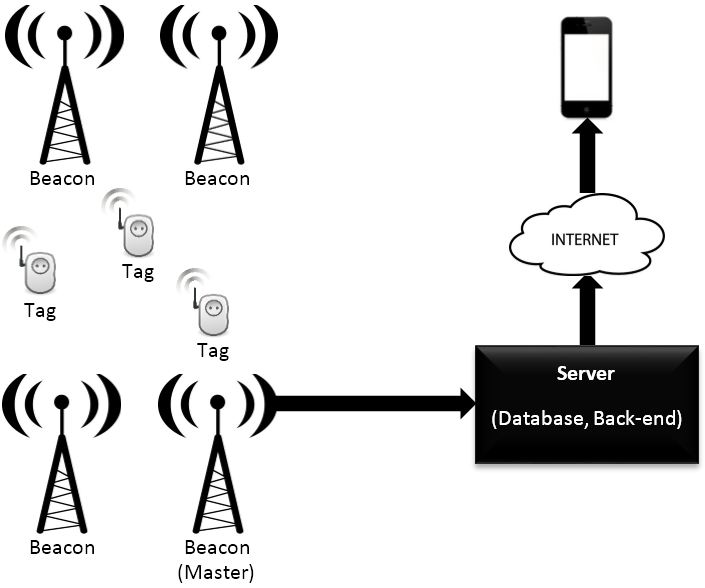
\includegraphics[scale=0.5]{data/software/1.jpg}
\caption{System overview.}
\label{fig:soft-overview}
\end{center}
\end{figure}

\newpage
\subsection{Software Design}
This section will cover aspects relating to the software design of the system. Included is a detailed explanation of how the positions of tags will be determined. A simulation will be used to validate the algorithm and assess how distance error affects the positioning error. The format of the packets that the tags send out will be established, and the back-end database design will be presented.

\subsubsection{Positioning using Trilateration} \label{trilateration}
Trilateration is a geometric process by which the coordinates of a point of interest can be determined by measuring the distance from that point to at least three other known reference points. In the two dimensional case (which we will consider for relatively level parking areas), each distance measurement corresponds to the radius of a circle centred at its respective reference point. The unknown point of interest is located at the intersection point of the three circles.
Figure 6.3.2-1 below illustrates the process. P1, P2 and P3 are known reference points at respective distances r1, r2 and r3 from the point of interest, B. It is clear why a minimum of three reference points are needed. If only one reference point is used, the point of interest could be located anywhere on the circumference of the circle around the point. If two reference points are used (P1 and P2, for example), the resulting circles drawn intersect at a maximum of two places – points A and B in the figure. A third reference point is required to narrow down the possible locations to one.
In the parking system application, the point of interest is a vehicle (specifically, the tag inside the vehicle), and each beacon is a reference point. It should be noted that although only three beacons are required, a fourth beacon is added to the final system for redundancy. 

\begin{figure}[H]
\begin{center}
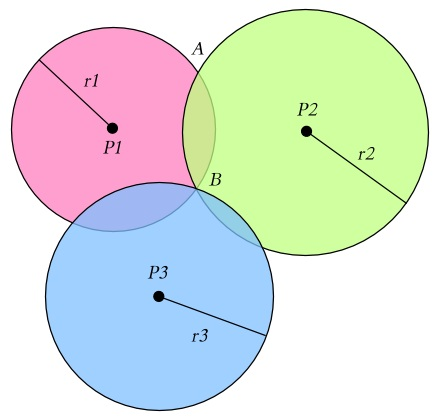
\includegraphics[scale=0.6]{data/software/2.jpg}
\caption{Process of trilateration.\cite{4}}
\label{fig:trilateration}
\end{center}
\end{figure}

\newpage
The means by which the tag's distance to each beacon is determined will now be explained. It is noteworthy that there are multiple methods to estimate the required distance in this application. A few alternatives will briefly be discussed, and the final selection will be expanded upon.

\lsec{Received Signal Strength Technique}
The first method to be discussed is one which uses the received signal strength (RSS) of the signal. Since the energy of the transmitted signal is known, and the energy of the received signal can be determined at the beacons, an estimate of the distance which the signal has travelled can be calculated. However, this requires the assumption of the path loss exponent n. Unfortunately, the value of n can vary, and an exceptionally accurate estimate of its value is needed in order to calculate the distance without any significant level of error. As a result, currently this technique cannot produce a mean accuracy of less than five metres.\cite{gaffney}

\lsec{Time of Flight Technique}
Another technique which can estimate the distance from the tag to the surrounding beacons uses an estimate of the time of flight of the transmitted packet. If the transmission time at the tag and the arrival time at the beacon are known, then the distance between the two can trivially be determined since the propagation speed of the signal is the speed of light. With the assumption that the clocks in the tags and the beacons are synchronized, this method can yield very accurate estimates of the distance. However, crystal effects mean that the clocks will drift with respect to each other over time.\cite{gaffney} This can be combated by periodically sending out clock synchronization packets to the tags, but this is not viable for this application because the tags are to be designed only to periodically transmit and never receive. This is a strict requirement put in place in order to ensure a sufficiently long battery life for the tags. Therefore, this alternative is not suitable.

\lsec{Time Difference of Arrival Technique}
The final technique to be discussed is a modification to the previous method described above. As previously stated, the location of a tag can be determined by finding the intersection of three circles, each centred at a beacon. The radius of each circle is the distance, given by the product of the time of flight of the transmitted signal and the speed of light. The equations of the three circles are as follows\cite{gaffney}:

$$(\tau_1 c)^2 = (x_1-x_t)^2 + (y_1-y_t)^2$$
$$(\tau_2 c)^2 = (x_2-x_t)^2 + (y_2-y_t)^2$$
$$(\tau_3 c)^2 = (x_3-x_t)^2 + (y_3-y_t)^2$$
Where:
\begin{itemize}
\item $\tau_n$ is the time of flight between the tag and the beacon n,
\item $c$ is the speed of light,
\item $(x_n,y_n)$ is the location of beacon n, which is known, and
\item $(x_t,y_t)$ is the location of the tag, which is unknown.
\end{itemize}

\newpage
Solving the intersection of the above equations will allow the determination of the location of the tag. The problem is that with tags using clocks which are unsynchronized with the beacons, the time of flights $\tau_n$ cannot be determined.

The solution is the time difference of arrival (TDOA) technique. This technique is also known as multilateration. It computes the time difference of arrival of a packet transmitted from the tag to the beacons. Only the beacons are assumed to have synchronized clocks. This technique will now be demonstrated.

Assume that at a time $t_0$, a tag transmits a packet. Beacons 1, 2 and 3 each receive the packet at times $t_1$, $t_2$ and $t_3$ respectively. The time of flights are then given by the equations below:

$$\tau_1 = t_1 - t_0$$
$$\tau_2 = t_2 - t_0$$
$$\tau_3 = t_3 - t_0$$

Allow the time difference of arrival (or the difference in the time of flight) between beacon 1 and beacon 2 to be $\Delta \tau_{12}$. By definition, it is given by the following equation:

\begin{equation*}
\begin{split}
\Delta \tau_{12} &= \tau_1 - \tau_2\\
 &= t_1 - t_0 - t_2 + t_0\\
 &= t_1 - t_2\\
\end{split}
\end{equation*}

Taking beacon 3 as the system origin and defining its position as (0, 0), it can be written that:

\begin{equation*}
\begin{split}
\Delta \tau_{13} &= \frac{1}{c} \sqrt{(x_1-x_t)^2 + (y_1-y_t)^2} - \frac{1}{c} \sqrt{(x_3-x_t)^2 + (y_3-y_t)^2}\\ 
&= \frac{1}{c} (\sqrt{(x_1-x_t)^2 + (y_1-y_t)^2} - \sqrt{x_t^2 + y_t^2})
\end{split}
\end{equation*}

\begin{equation*}
\begin{split}
\Delta \tau_{23} &= \frac{1}{c} \sqrt{(x_2-x_t)^2 + (y_2-y_t)^2} - \frac{1}{c} \sqrt{(x_3-x_t)^2 + (y_3-y_t)^2}\\ 
&= \frac{1}{c} (\sqrt{(x_2-x_t)^2 + (y_2-y_t)^2} - \sqrt{x_t^2 + y_t^2})
\end{split}
\end{equation*}

The equations above define two hyperbolae - the intersection of which gives the tag location (xt,yt).\cite{gaffney}

\newpage
\subsubsection{Simulation}

While the TDOA method described above is mathematically sound, it is somewhat unknown what the positioning accuracy will be in the real world with error caused by signal attenuation and other factors which have been thus far ignored. In order to better visualize the accuracy and effectiveness of the TDOA trilateration technique, a simple simulation was programmed in C\#. Figure~\ref{fig:distance-error} shows a screenshot of the running simulation.

\begin{figure}[H]
\begin{center}
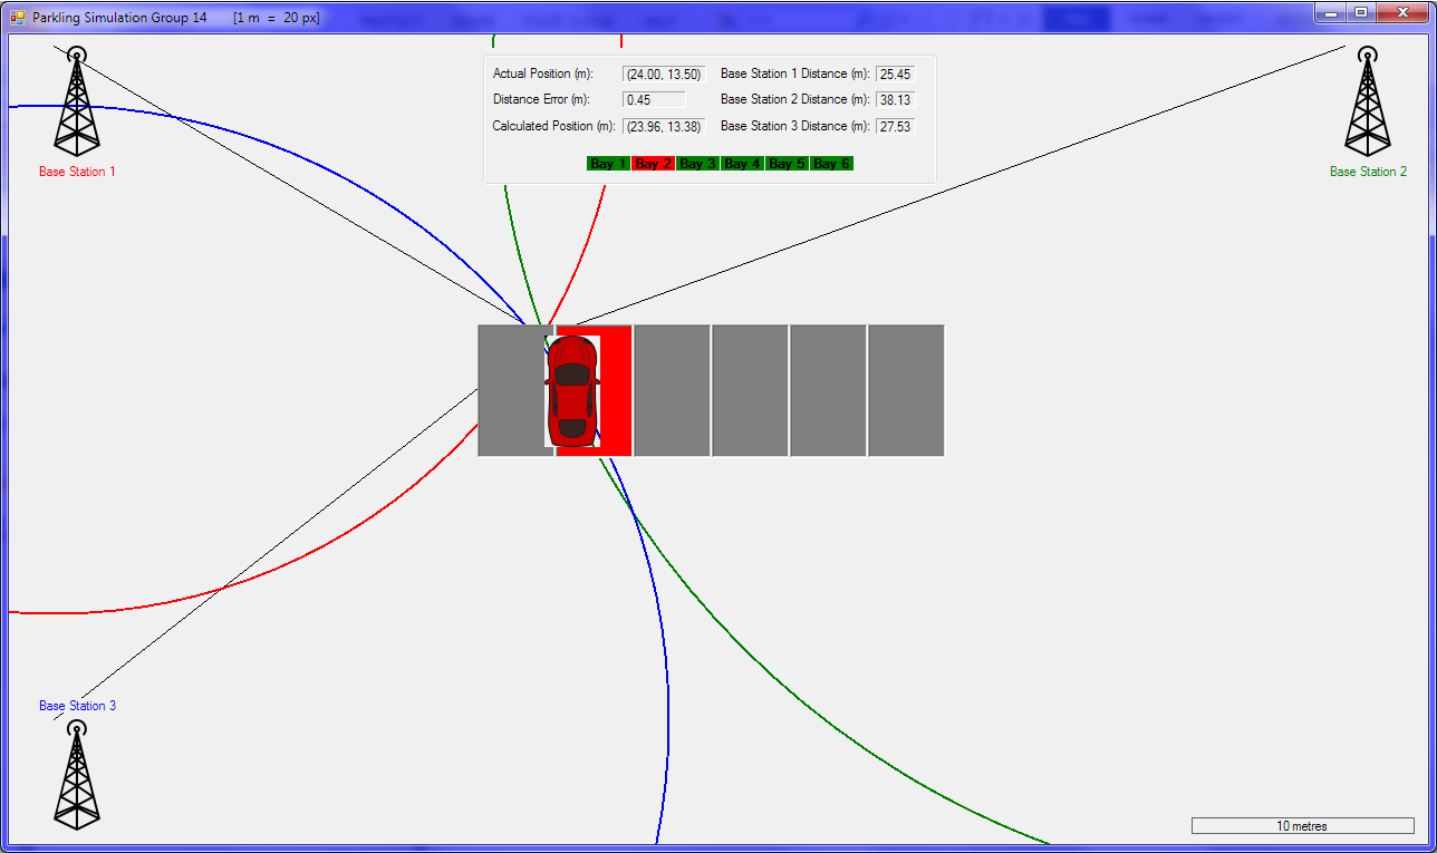
\includegraphics[scale=0.4]{data/software/3.jpg}
\caption{Simulation used to test the effect of distance error on positioning accuracy.}
\label{fig:distance-error}
\end{center}
\end{figure}

\lsec{Simulation Algorithm}
The simulation determines the position of a vehicle and checks whether it is in a parking bay according to the following, simplified algorithm:

\begin{enumerate}
\item The exact distance from the vehicle to each of the beacons is determined geometrically.
\item A random error with adjustable maximum scale (in the range from 0 - 1 m) is introduced into each of the three distance measurements.
\item The two intersection points of the circles centred at beacons 1 and 2 are determined.
\item The intersection point closest to beacon 3 is taken as the location of the vehicle.
\item The simulation checks whether the calculated location is in the region of any of the parking bays.
\end{enumerate}

\newpage
\lsec{Sources of Error}
Clock drift introduces an insignificant error in the TDOA trilateration technique (as long as the beacons are synchronized often enough). Another source of error comes from the fact that, effectively, the reported distance varies slightly (as figure~\ref{fig:reported-distance} shows) according to the received signal level. This error could be sufficiently large to become problematic for the parking system application. However, it can be compensated for using Friis' well-known path loss formula.\cite{2}

\begin{figure}[H]
\begin{center}
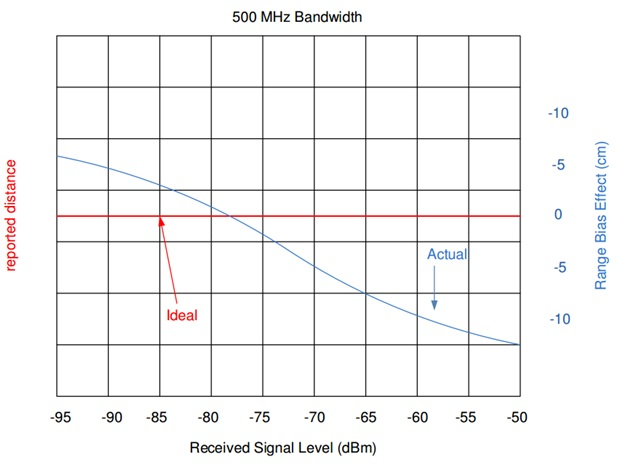
\includegraphics[scale=0.8]{data/software/4.jpg}
\caption{The effect of received signal level on the reported distance.\cite{2}}
\label{fig:reported-distance}
\end{center}
\end{figure}

The only remaining potentially significant source of error is that caused by signal attenuation resulting from the tag's transmission having to pass through at least one vehicle body and potentially other obstacles. This can be minimised by ensuring that the beacons are high enough above ground level (to minimize the number of vehicle bodies that the signal must propagate through) and maintaining the surrounding area (by trimming foliage and clearing other obstacles). Regardless, some error will be introduced into the system, and the simulation was used to determine the effect of distance error.

\lsec{Findings of the Simulation}
The simulation revealed that the system was surprisingly tolerant to errors in distance. Using a distance error with a maximum magnitude below 0.50 m, even a car parked partially (about 15\%) in another bay was detected correctly 100\% of the time. Since the error introduced by variation in the received signal level can be nearly eradicated using Friis' path loss formula, it is concluded that the system will be accurate enough, with the assumption that the distance error will be less than 0.50 m. This appears to be a very safe assumption as the DecaWave chips are quoted as giving a positioning accuracy up to 0.10 m indoors.\cite{3}

\newpage
\subsubsection{Tag Packet Format} \label{tag-packet}
This subsection will briefly outline and justify the contents of the packets that tags will emit. Each data packet will have the following data:

\begin{itemize}
\item The ID of the tag – to identify the tag and therefore vehicle and user.
\item Time the packet was transmitted – to be used in the TDOA calculation.
\item Battery level of the tag – to inform the user via the app/email/SMS that the battery is low.
\end{itemize}

These packets will be periodically transmitted by each tag every 5-10 minutes in order to conserve their battery life.

\subsubsection{Database Design}
This subsection will detail the design of the parking system database. Specifically, the design of each of the three main tables required to make the system work is presented and explained. The three main tables are:

\begin{itemize}
\item Parking Areas
\item Parking Bays
\item Tags
\end{itemize}

The design of these tables will be expanded upon below:

\lsec{Parking Areas}

\begin{table}[H]
\begin{center}
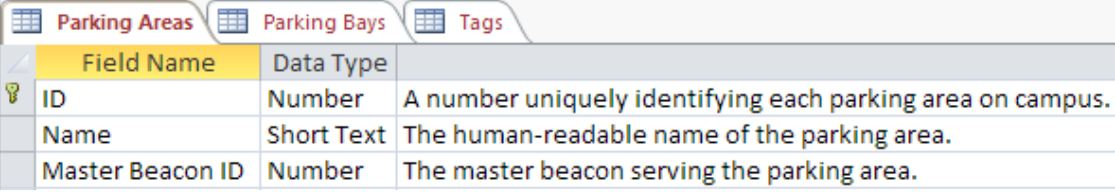
\includegraphics[scale=0.5]{data/software/5.jpg}
\caption{Parking Areas table.}
\label{tbl:table-parking-areas}
\end{center}
\end{table}

Table~\ref{tbl:table-parking-areas} shows the design of the Parking Areas table. This is a simple table in which each parking area has a record. The purpose of the Master Beacon ID field is so that the server knows which parking area the information it receives relates to, based on which master beacon it received the information from.

\newpage
\lsec{Parking Bays}

\begin{table}[H]
\begin{center}
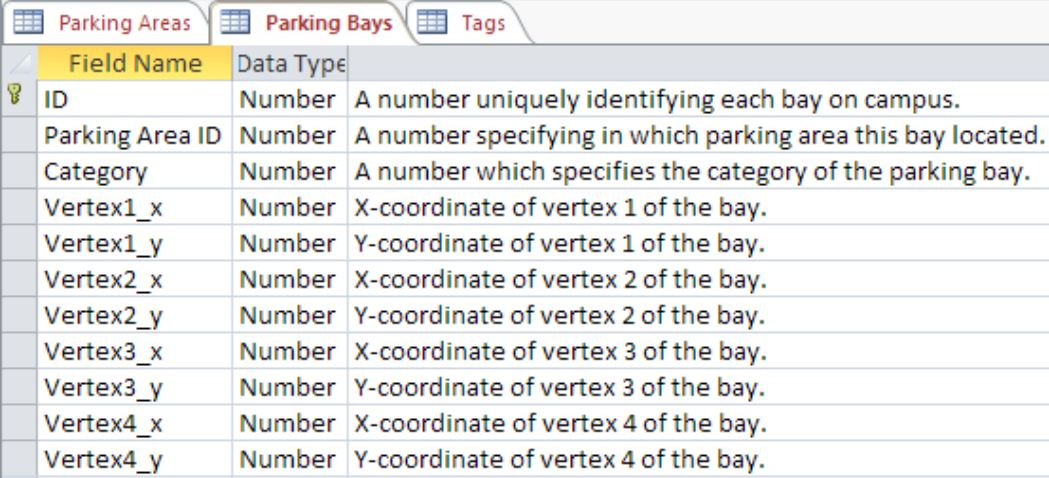
\includegraphics[scale=0.5]{data/software/6.jpg}
\caption{Parking Bays table.}
\label{tbl:table-parking-bays}
\end{center}
\end{table}

Table~\ref{tbl:table-parking-bays} shows the design of the Parking Bays table. Every single parking bay on campus will be entered as a record in this table. The Parking Area ID field details in which parking area each bay is located. The category field can be updated via the traffic department's client app as required. For example, student bays could be reassigned to be postgraduate bays. The eight vertex fields define the coordinates of each of the four corners of the parking bay. This is used to determine which bay a tag is occupying, if any.

\lsec{Tags}

\begin{table}[H]
\begin{center}
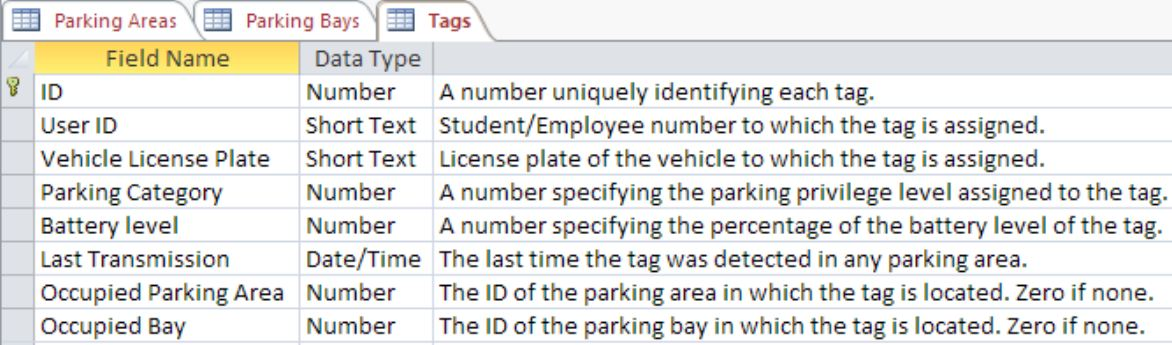
\includegraphics[scale=0.5]{data/software/7.jpg}
\caption{Tags table.}
\label{tbl:table-tags}
\end{center}
\end{table}

Table~\ref{tbl:table-tags} shows the design of the Tags table. The design of this table takes into consideration that a single user may have multiple vehicles and therefore multiple assigned tags, but the tag-vehicle relationship is one-to-one. This means that each tag can only be assigned to one vehicle, and a vehicle can only have one tag assigned to it.

\newpage
The parking category field is used to determine whether the user is allowed to park a specific tag/vehicle in any given bay. The tag's reported battery level is stored in order to notify the user via the mobile app/email/SMS that the battery is low and needs to be replaced.
The Last Transmission field is used for statistics to keep track of how long users spend on campus.

\subsubsection{Mobile and Web Application}

This subsection will briefly outline the functionality of the mobile and web application. The two applications will have the same features. Each user logs in with their student/employee number and UCT password. There will be only one type of app, regardless of the user type. There will be three user types:

\lsec{Admin Users}
These users are able to control the assignment of parking bay categories. They also have access to statistical information that can be used to monitor patterns on campus in order to improve the parking system.

\lsec{Traffic Officials}
These users have the ability to view the location of illegally parked cars and mark them once they have been fined or clamped.

\lsec{Parking Users}
These users receive information about parking availability (via their smartphone's screen, or a synthesized voice to allow operation while driving) according to their assigned parking category and preferred parking areas. They will also be given an estimated time (determined from historical data) by which they must arrive on campus if they wish to park in their preferred parking area.

The parking users will be informed if they have parked illegally, been fined or clamped. They will be able to view the last location and battery status of each of their vehicles/tags, provided the tags are located in a parking area on campus.

\newpage
\subsection{Mechanical Design} 
\subsubsection{Mechanical Requirements}
Durability, forces, dynamics.
\subsubsection{Technical Drawings}
\subsection{Electrical Design} 
\subsubsection{Power Requirements}
Battery life etc.

\newpage
\subsubsection{Schematics}

The following diagrams cover the design of the tag; where the beacon makes a few changes to the circuitry and adds a WiFi module, seen in Figure~\ref{fig:wifi}.

\begin{figure}[H]
\begin{center}
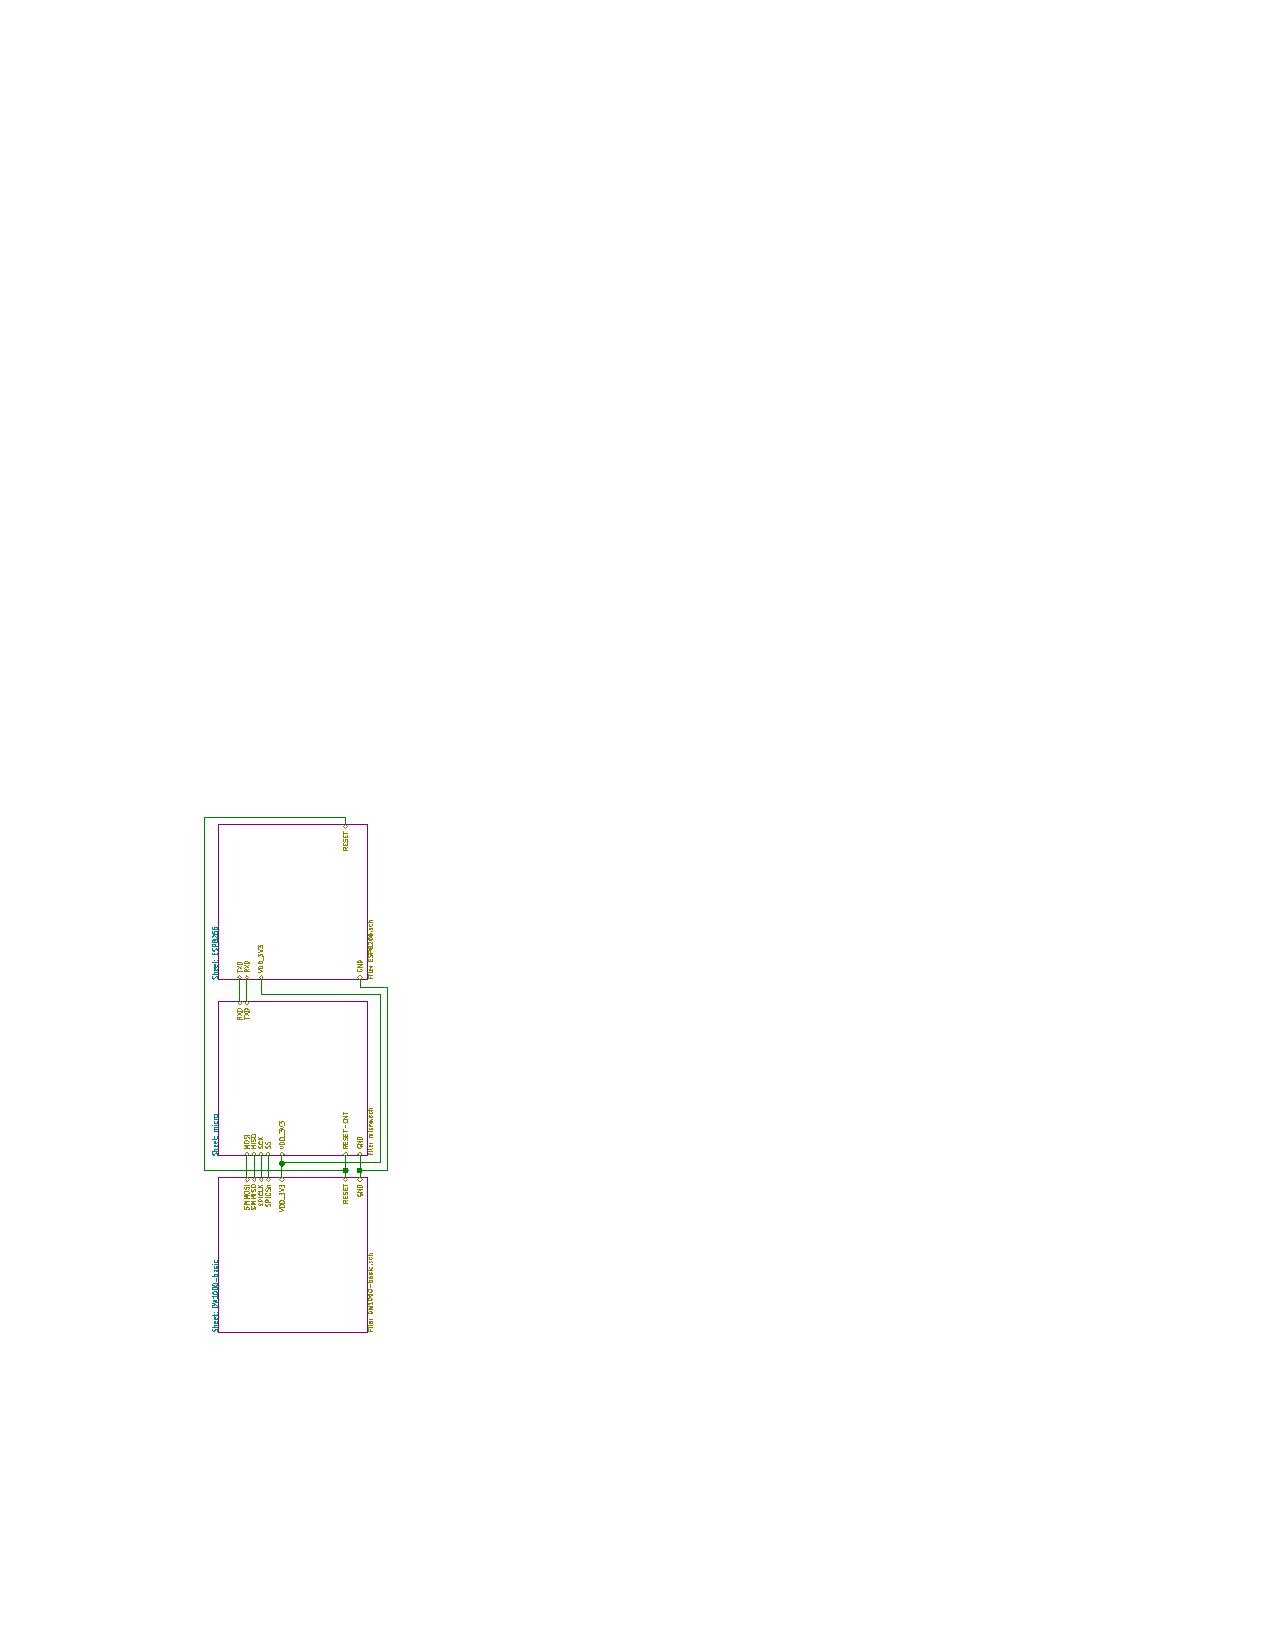
\includegraphics[page=1,scale=1.5,trim={3cm 5cm 15cm 13cm},clip,angle=-90]{data/parking-system2.pdf}
\caption{Parking system tag schematic diagram: interface connections.}
\end{center}
\end{figure}

\begin{figure}[H]
\begin{center}
\includegraphics[page=2,scale=0.5,trim={0cm 0cm 0cm 0cm},clip]{data/parking-system.pdf}
\caption{Parking system tag schematic diagram: transceiver chip.}
\end{center}
\end{figure}

\begin{figure}[H]
\begin{center}
\includegraphics[page=3,scale=1,trim={10cm 8cm 10cm 5cm},clip]{data/parking-system.pdf}
\caption{Parking system tag schematic diagram: micro-controller.}
\end{center}
\end{figure}

\begin{figure}[H]
\begin{center}
\includegraphics[page=4,scale=1,trim={5cm 9cm 10cm 13cm},clip,angle=-90]{data/parking-system2.pdf}
\caption{Parking system beacon schematic diagram: WiFi module.}
\label{fig:wifi}
\end{center}
\end{figure}

\newpage
\subsubsection{PCB Design}

EMF and RF mitigation techniques have to be considered when designing the PCBs in order to make them compliant with the ICASA regulations. This involved using a ground plane and ensuring the antennas are correctly matched ($100\Omega$ traces) to reduce RF harmonic signals.

\begin{figure}[H]
\begin{center}
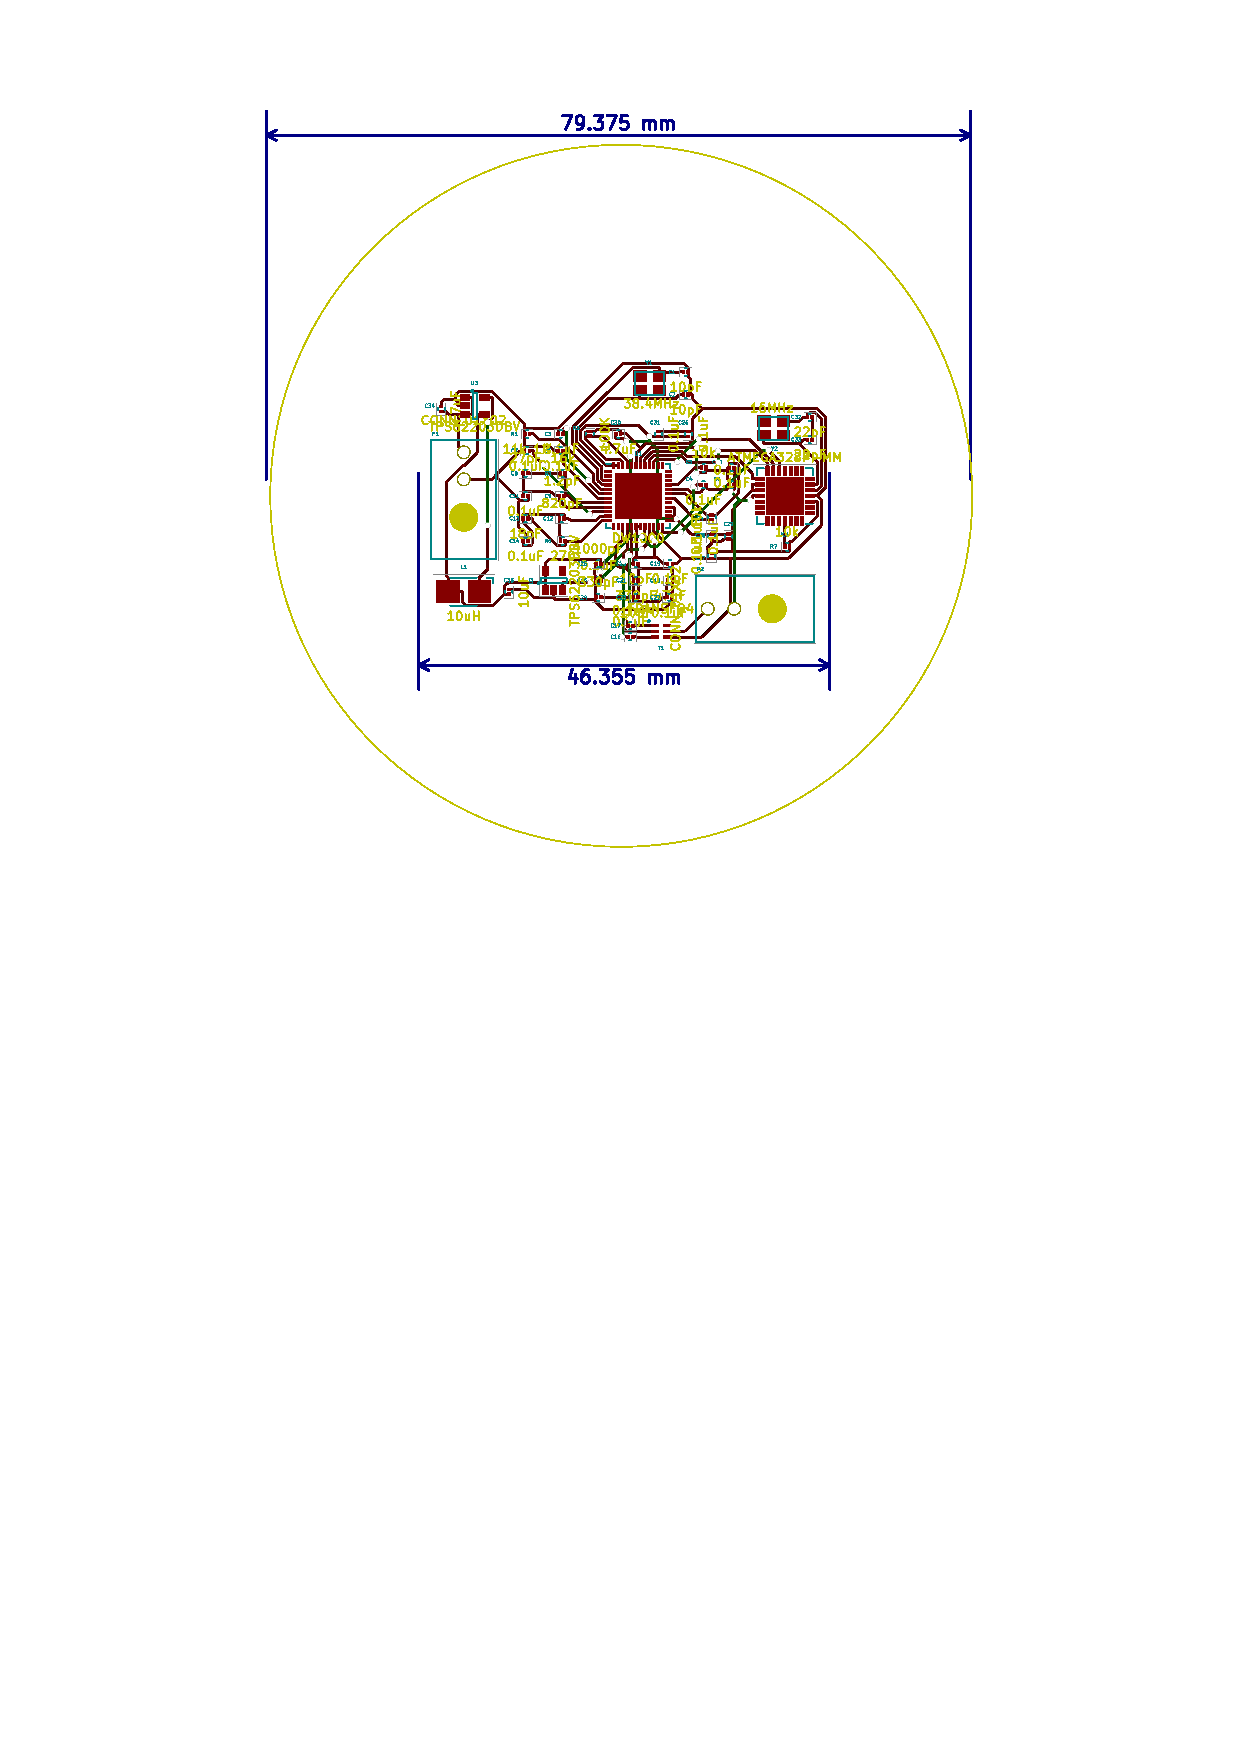
\includegraphics[scale=0.7,trim={4cm 15cm 4cm 1cm},clip]{data/pcb-layout.pdf}
\caption{Parking system tag PCB layout.}
\end{center}
\end{figure}

\begin{figure}[H]
\begin{center}
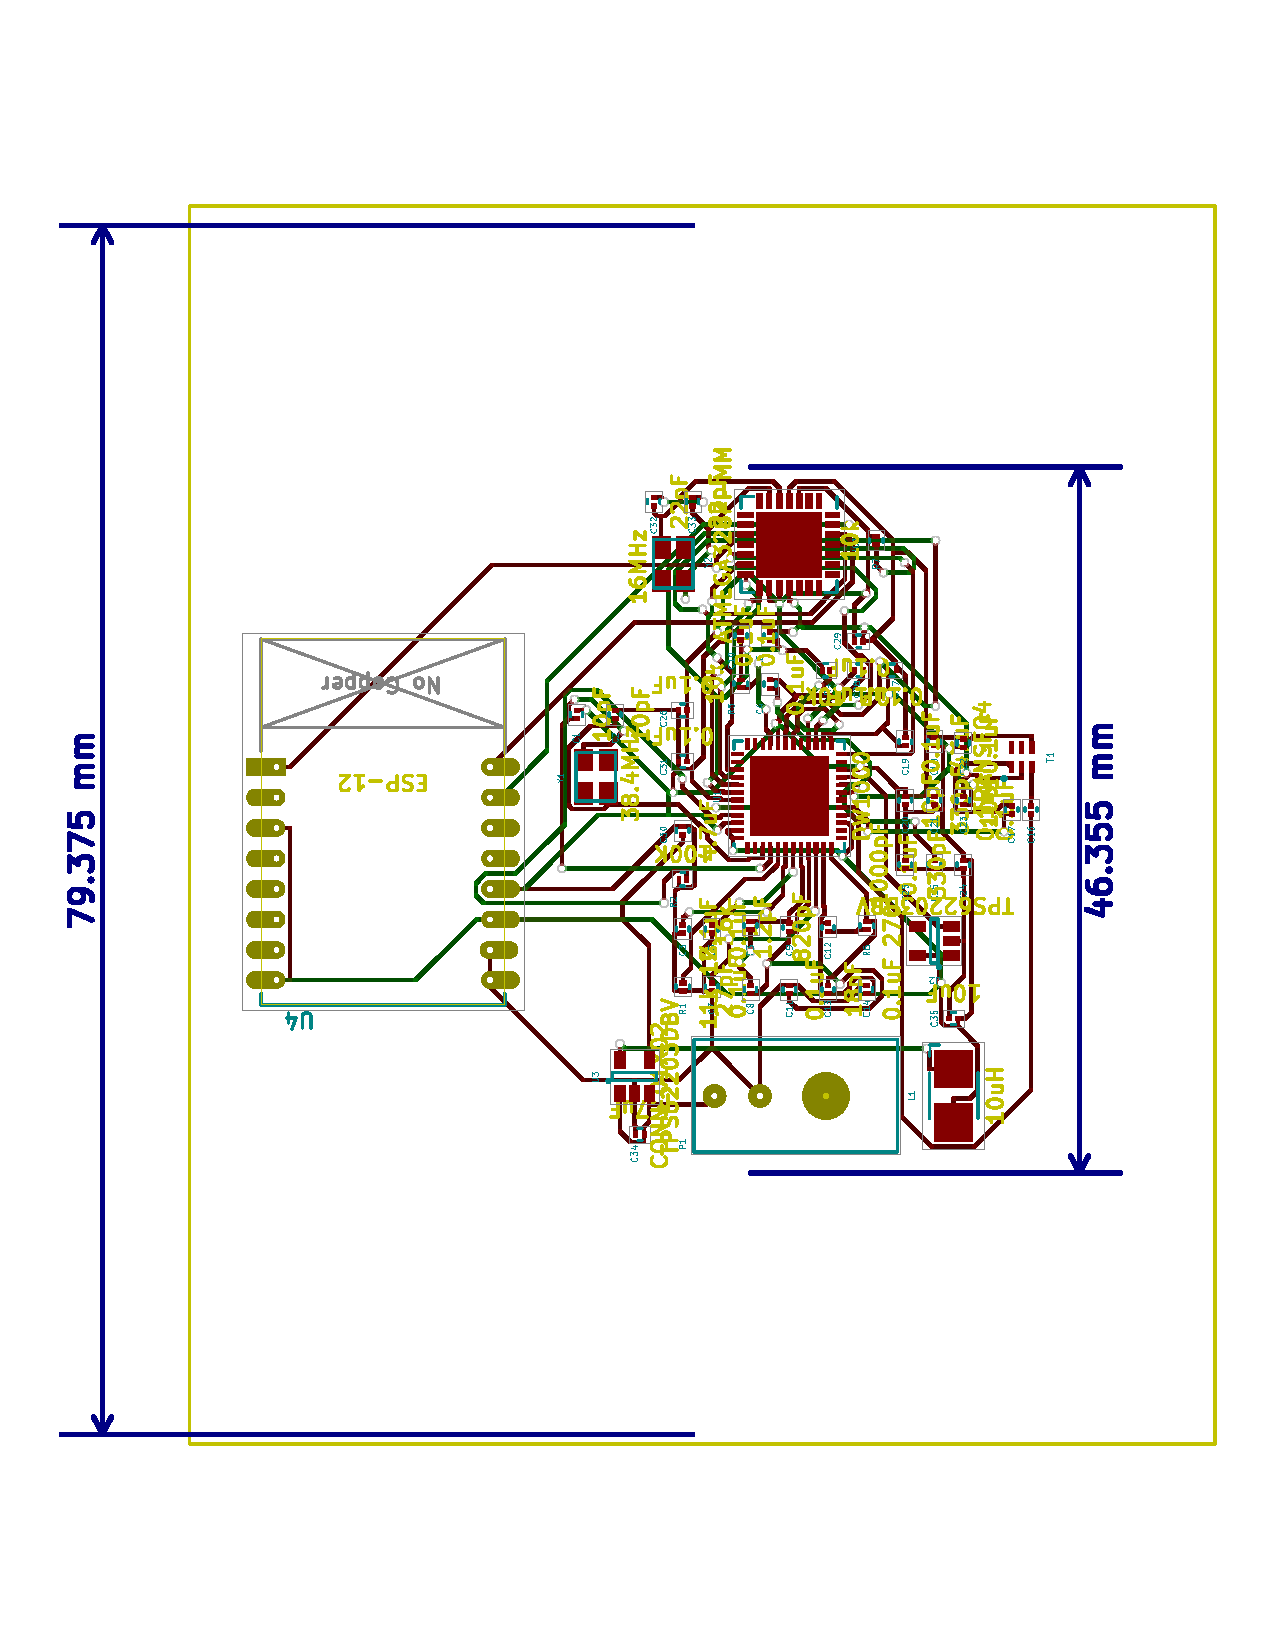
\includegraphics[scale=0.4,trim={1cm 1cm 1cm 1cm},clip,angle=-90]{data/pcb-layout-ESP.pdf}
\caption{Parking system beacon PCB layout.}
\end{center}
\end{figure}



\newpage
\subsubsection{RF Design}


\lsec{Antenna Specifications:\cite{DW-antenna}}

Friis' Transmission Equation states the following:
$$P_{RX} = \frac{P_{TX}G_{TX}G_{RX} \lambda^2}{(4 \pi r)^2}$$
There is a quadratic relationship between the received power ($P_{RX}$) and the distance r from the tag to the beacon. This means we need to optimize the received power in another way, as the distance r can not be optimized except by having a dense beacon installation. The transmit power ($P_{TX}$) needs to be kept as low as possible, to optimize battery usage - this means the transmit and received antenna gain need to be made as high as is possible. The tag has a limited space profile, which means the beacon antenna needs to be as large as possible. Unfortunately the beacon antenna needs to be fairly omni-directional in order to pick up all the tags, as will be explained below, this further limits the possible receiver gain.

Because the antenna gains are measured using decibels which are on a logarithmic scale, the following form of the equation needs to be used:

$$P_{RX} = P_{TX} + G_{TX} + G_{RX} + 20log_{10}(\frac{\lambda}{4 \pi R})$$


We would like to achieve at least a 60 percent transmission efficiency (this means 60 percent of the transmitted power is received) with a target of 90 percent efficiency. Designing for a 75 percent efficiency will help us achieve this target: 

$$\lambda = \frac{300e6}{f} = \frac{300e6}{3GHz} = 0.1m$$

$$EIRP(f) = P_{TX}G_{TX} = -41.3dBm/MHz$$
\begin{center}
value as mentioned below in regulations. This means the peak transmitter power and peak transmitter antenna gain must give a product within the regulations.
\end{center}

The typical transmit power level for $P_{TX}$ is 35dB.\cite{DW-data} The $G_{TX}$ rating for the tag chip antenna chosen is 2.6dBi.

Using the logarithmic form of Friis' Transmission Equation, we find the following value for the receiver gain: 
$$10log_{10}(0.75) \times 35dB = 35dB + 2.6dBi + G_{RX} + 20log_{10}(\frac{0.1}{4 \pi \times 200})$$
$$G_{RX} = 6.68dBi$$
Because the receiver antenna will have a vertically polarised dipole radiation pattern to maximise  gain, the value for $G_{RX}$ with relation to a dipole antenna is:\cite{Book-Antenna} 
$$G_{RX} = 6.68dBi - 2.15dB = 4.53dBd$$

\begin{table}[H]
\centering
\caption{Antenna specifications: tag and beacon}
\label{antenna-specs}
\begin{tabular}{l l l l}
\textbf{Aspect}                      & \textbf{Tag} & \textbf{Beacon} \\ 
Radiation Pattern    	& Isotropic             & Dipole              \\
Power Output (EIRP)		& $-41.3dBm/MHz$ or 35dB        & N/A \\
Gain (TX and RX resp.)                	& 2.6dBi                     & 4.53dBd                    \\
Physical Area 			& 8mm length					 & $1m^2$          \\         
Location 				& Mobile                & Fixed                    \\         
\end{tabular}
\end{table}

\lsec{Tag Antenna Choice}
The tag antenna specifications are based on the calculations above and using the AH086M555003 PCB chip antenna from Mouser which has a wide operating range from 3100MHz to 8000MHz. In the calculations above it is clear to see that a transmission gain of 2.6dBi is more than enough for a reasonable receiver gain to be found. The chip antenna chosen is small enough to fit the specified area on the PCB.

PCB antennae require more complex PCB design and placement to achieve the same performance as chip antennae. Chip antennae require matching circuitry that affect the performance greatly - chip antennae are capable of performing favourably in the right conditions, with a near isotropic radiation pattern as required.\cite{TI-Ant}

\lsec{Beacon Antenna Choice}
A vertically polarised 1/4 wavelength dipole antenna will be used. This will give a uniform radiation pattern in the horizontal plane as required, and a gain of 4.53dBd is easily achieved. There is no size constraint especially with the high frequency being used and the fixed environment, so if a higher gain is needed multiple directional antennae could be implemented.

\lsec{ICASA National Radio Frequency Plan:\cite{ICASA}\cite{UWB-Regs}}
The ICASA 2013 NRFP for ITU Region 1 allocates the frequency range from 3.3GHz to 3.4GHz to radio-location with a typical application of government services. In South Africa there are no specific regulations for UWB signals. The Decawave technology is ETSI compliant and will generally be accepted by ICASA so long as EMF and RF mitigation techniques are used. The regulations permit outdoor use on the frequency range 3.1-4.8GHz with an EIRP of -41.3dBm/MHz. The ETSI regulations permit the use of the Decawave chips in an indoor and outdoor environment.

\lsec{DW1000 Frequency Channels:\cite{DW-antenna}}
The DW1000 can be programmed to use specific frequency channels (defined by the IEEE 802.15.4a-2011 standard) with corresponding bandwidth. Based on the ICASA regulations above, Channel 1 would be used with a Centre Frequency of 3493.4MHz and an operational bandwidth of 500MHz. This falls within the informal regulations mentioned above. 

\lsec{Operating Range\cite{DW-manual}}
The operating range of the RF signal is affected by a number of software considerations. If a range of around 250m is required, slightly higher than the design constraint in the calculations above to allow for signal attenuation, then a data rate of 110kbps should be used on the tag side - for the beacon this is not critical as operating transmitter range and power use are less of a concern.

\newpage
\lsec{Further Design Considerations}
Further testing of antenna designs and power output will need to be done in the parking system environment as calculations can not be relied upon for RF design.

\begin{figure}[H]
\begin{center}
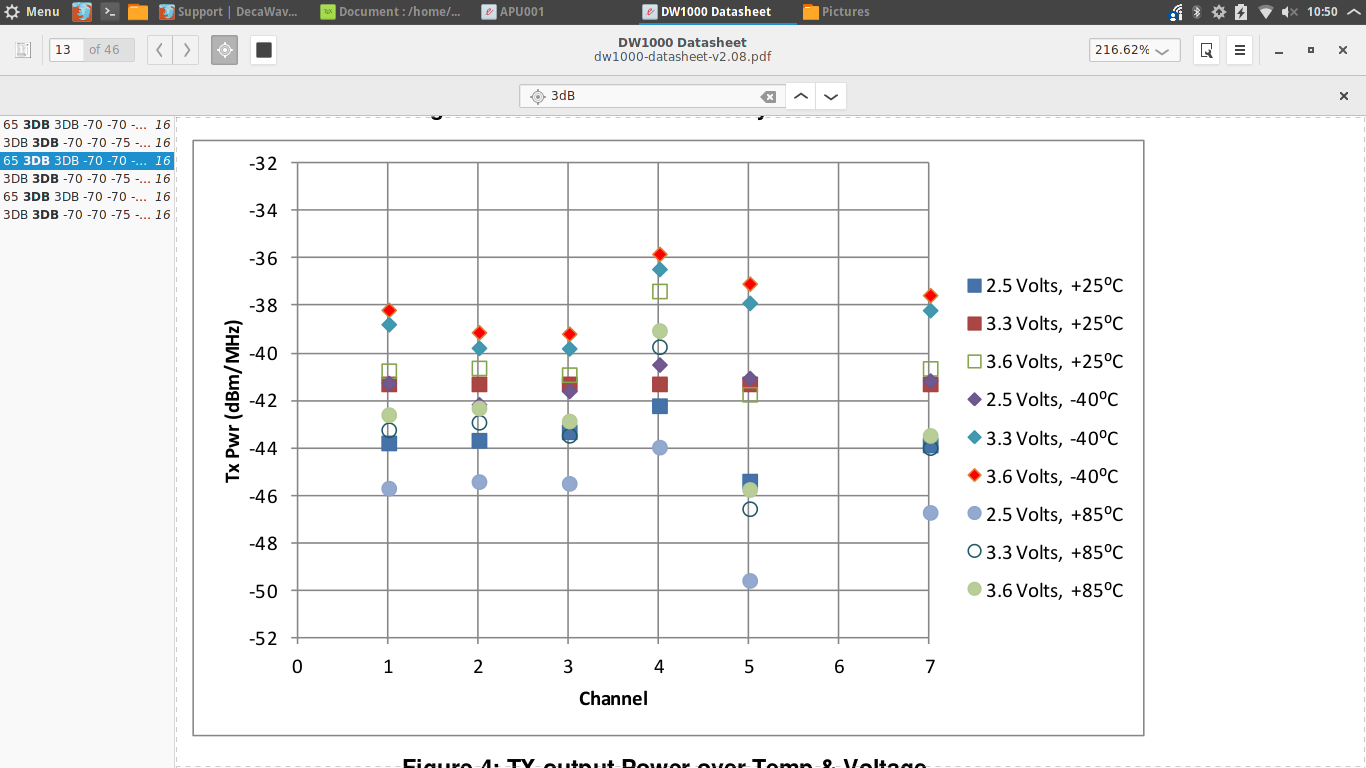
\includegraphics[scale=0.4,trim={7cm 1.5cm 8cm 5.5cm},clip]{data/tx_power.png}
\caption{TX Power vs Supply Voltage and Temperature.\cite{DW-data}}
\label{fig:tx-power}
\end{center}
\end{figure}

Figure~\ref{fig:tx-power} above shows that both the supply voltage and environmental temperature have an affect on the effective transmit power achieved. This means proper supply voltage regulation, as well as temperature regulation, are needed to ensure the transmit-receive performance designed for is achieved in practise.

\newpage
\subsubsection{Bill of Materials (Tag)}
The bill of materials as well as unit pricing for the tag can be found in Appendix F. Where parts with specific tolerance, such as for the RF circuitry, are needed they have been ordered specifically. The non-critical parts were chosen to optimize the end unit price. 

All parts were ordered from Mouser except if specified otherwise. They offer international shipping and are a reliable source of components to minimize risk. The LiPo batteries were ordered from a chinese source, as stated in the BOM, and the supplier will need to be managed properly to reduce risk.

\textbf{The result of the BOM and Unit Cost analysis is the following:}

Total Capital Outlay (ZAR): \\
Unit Cost (ZAR):

It was decided not to include the BOM and Unit Cost analysis for the beacons, as their costs will be minimal when compared with the 15000 tags needed for the system. In terms of circuitry, the beacons will work out to the same price as a tag - adding WiFi but not using LiPo batteries. There will be the additional expense of the following:

\begin{itemize}
\item WiFi chips
\item Beacon platform
\item Beacon power supplies
\item Antenna 
\end{itemize}

\subsection{Assumptions}
Identify and show that checked validity.
\subsection{Failure Modes}
Probabilities,Consequences,Mitigation
\subsection{System Lifetime}
A statement of the design life time, with explanation of what (if anything) will limit it.
\subsection{Worst Case Calculation}
For at least one component / sub-system 

\textit{Report structure compiled from class notes.}\cite{handout}\cite{notes}

%\begin{figure}[H]
%\begin{center}
%\includegraphics[trim={Lcm Bcm Rcm Tcm},clip]{images/Fig1.pdf}
%\caption{•}
%\end{center}
%\end{figure}

%\begin{minted}[linenos=true]{matlab}
%\end{minted}

%######################References######################
\newpage
%\input{"\homedir references.tex"} %manual references

\bibliography{bibliography}
\bibliographystyle{ieeetran}
\addcontentsline{toc}{section}{References}


%######################Appendices######################
\newpage
\vspace*{\fill}
\begin{center}
\subsection*{Appendix A: Contributions}
\end{center}
\vspace*{\fill}
\addcontentsline{toc}{section}{Appendix A: Contributions}

\newpage
\subsubsection*{Jarushen Govender (GVNJAR002)}
Progress Report 3.
\subsubsection*{Isaac Lebogang Khobo (KHBISA001)}
Progress Report 4.
\subsubsection*{Benjamin Scholtz (SCHBEN011)}
LATEX Formatting/Template. \\
2. Task Clarification. \\
3. Context of Design: Microeconomic Factors. \\
4. Design Specification: Scope, Applicable Documents, Quality Assurance, Timescale, Economic Factors, Ergonomic Factors, Life-cycle. \\
5. Conceptual Design: Design One, Weighted Selection, Recommendation. \\
6. Embodiment Design: Schematics, PCB Design, RF Design, Bill of Materials (Tag). \\
Progress Report 2.
\subsubsection*{Nasko Stavrev (STVATA001)}
Simulation.
6. Embodiment Design: System Overview, Software Design.

\vfill
\textbf{Note: }\textit{all team members contributed throughout the course of the design to the various sections mentioned - each section was compiled by the team member shown.}

\newpage
\vspace*{\fill}
\begin{center}
\subsection*{Appendix B: Progress Reports}
\end{center}
\vspace*{\fill}
\addcontentsline{toc}{section}{Appendix B: Progress Reports}

\newpage
\subsection*{Progress Report 1: SCHBEN011}
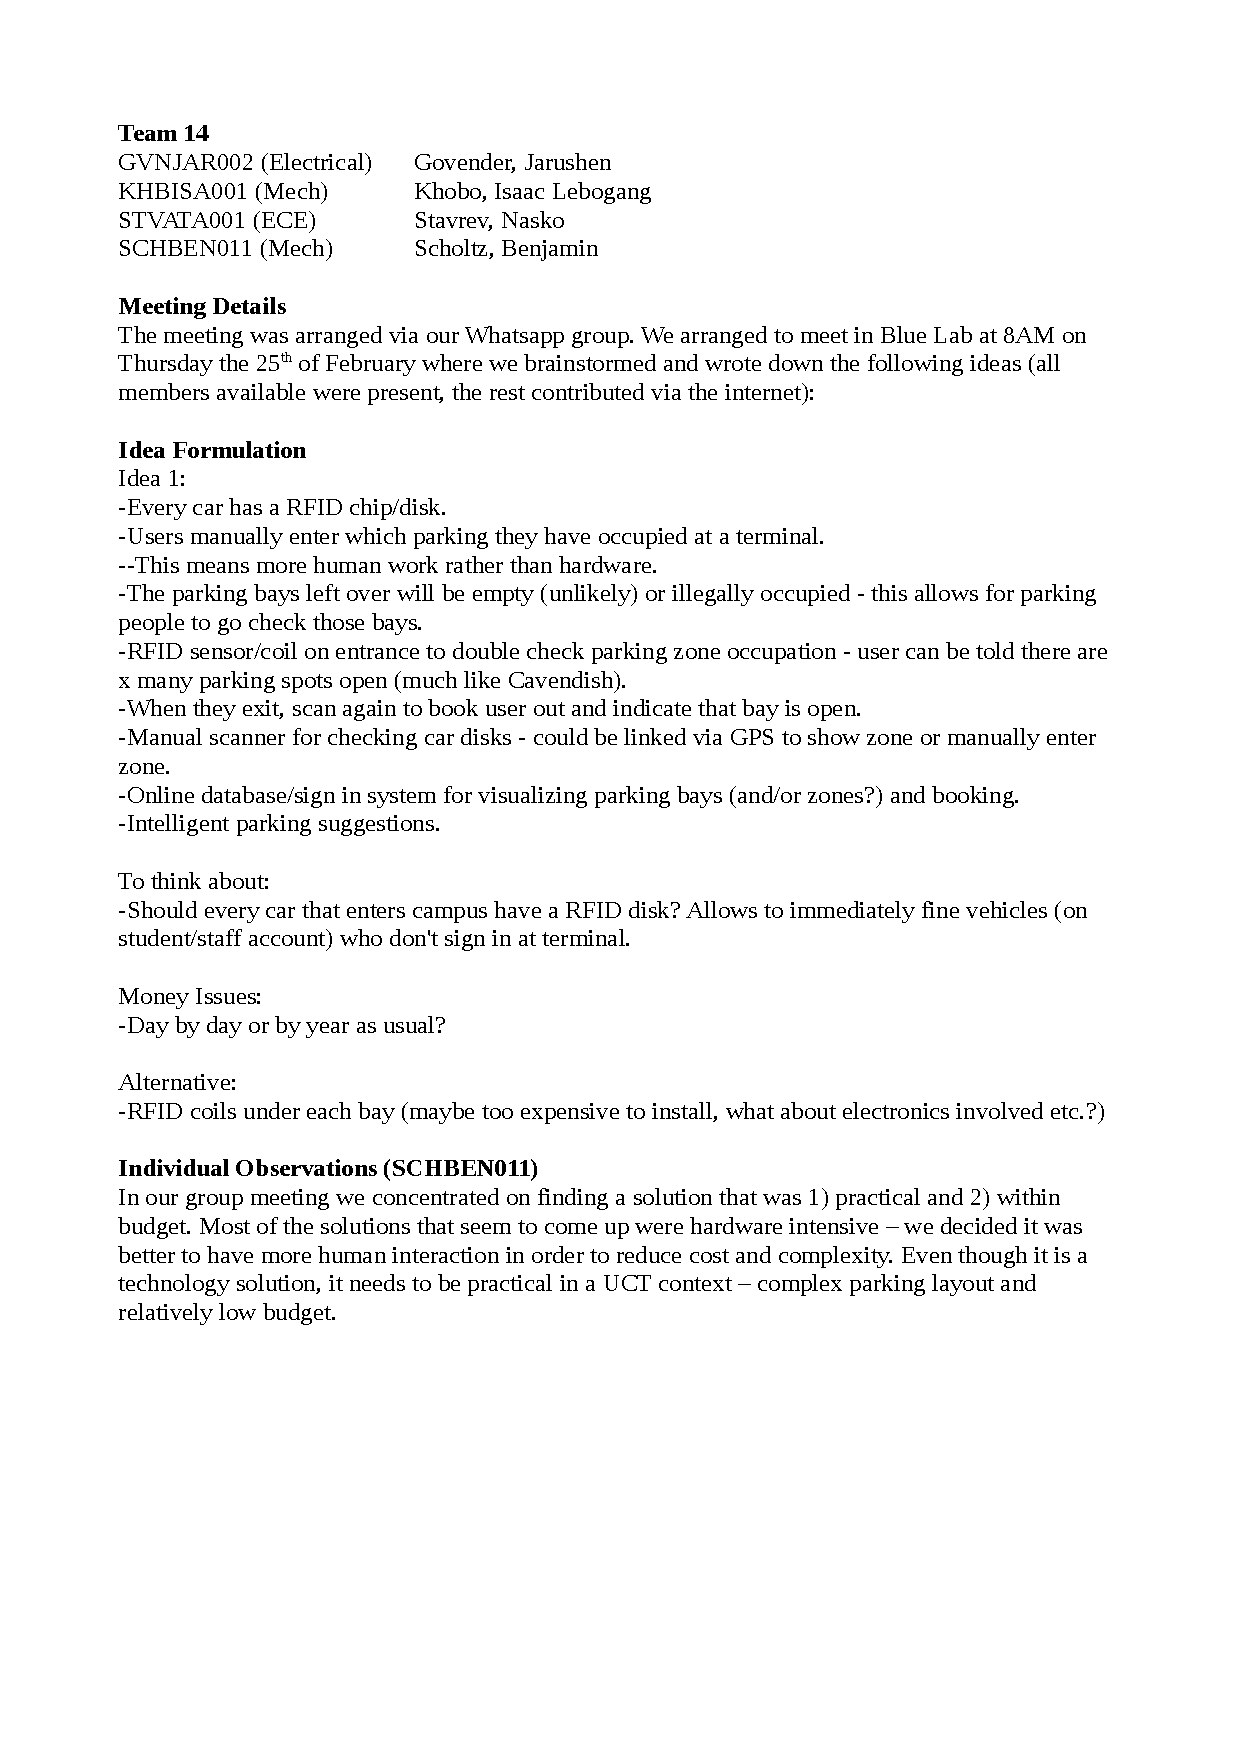
\includegraphics[scale=0.9]{meeting/report1-ben.pdf}

\newpage
\subsection*{Progress Report 1: STVATA001}
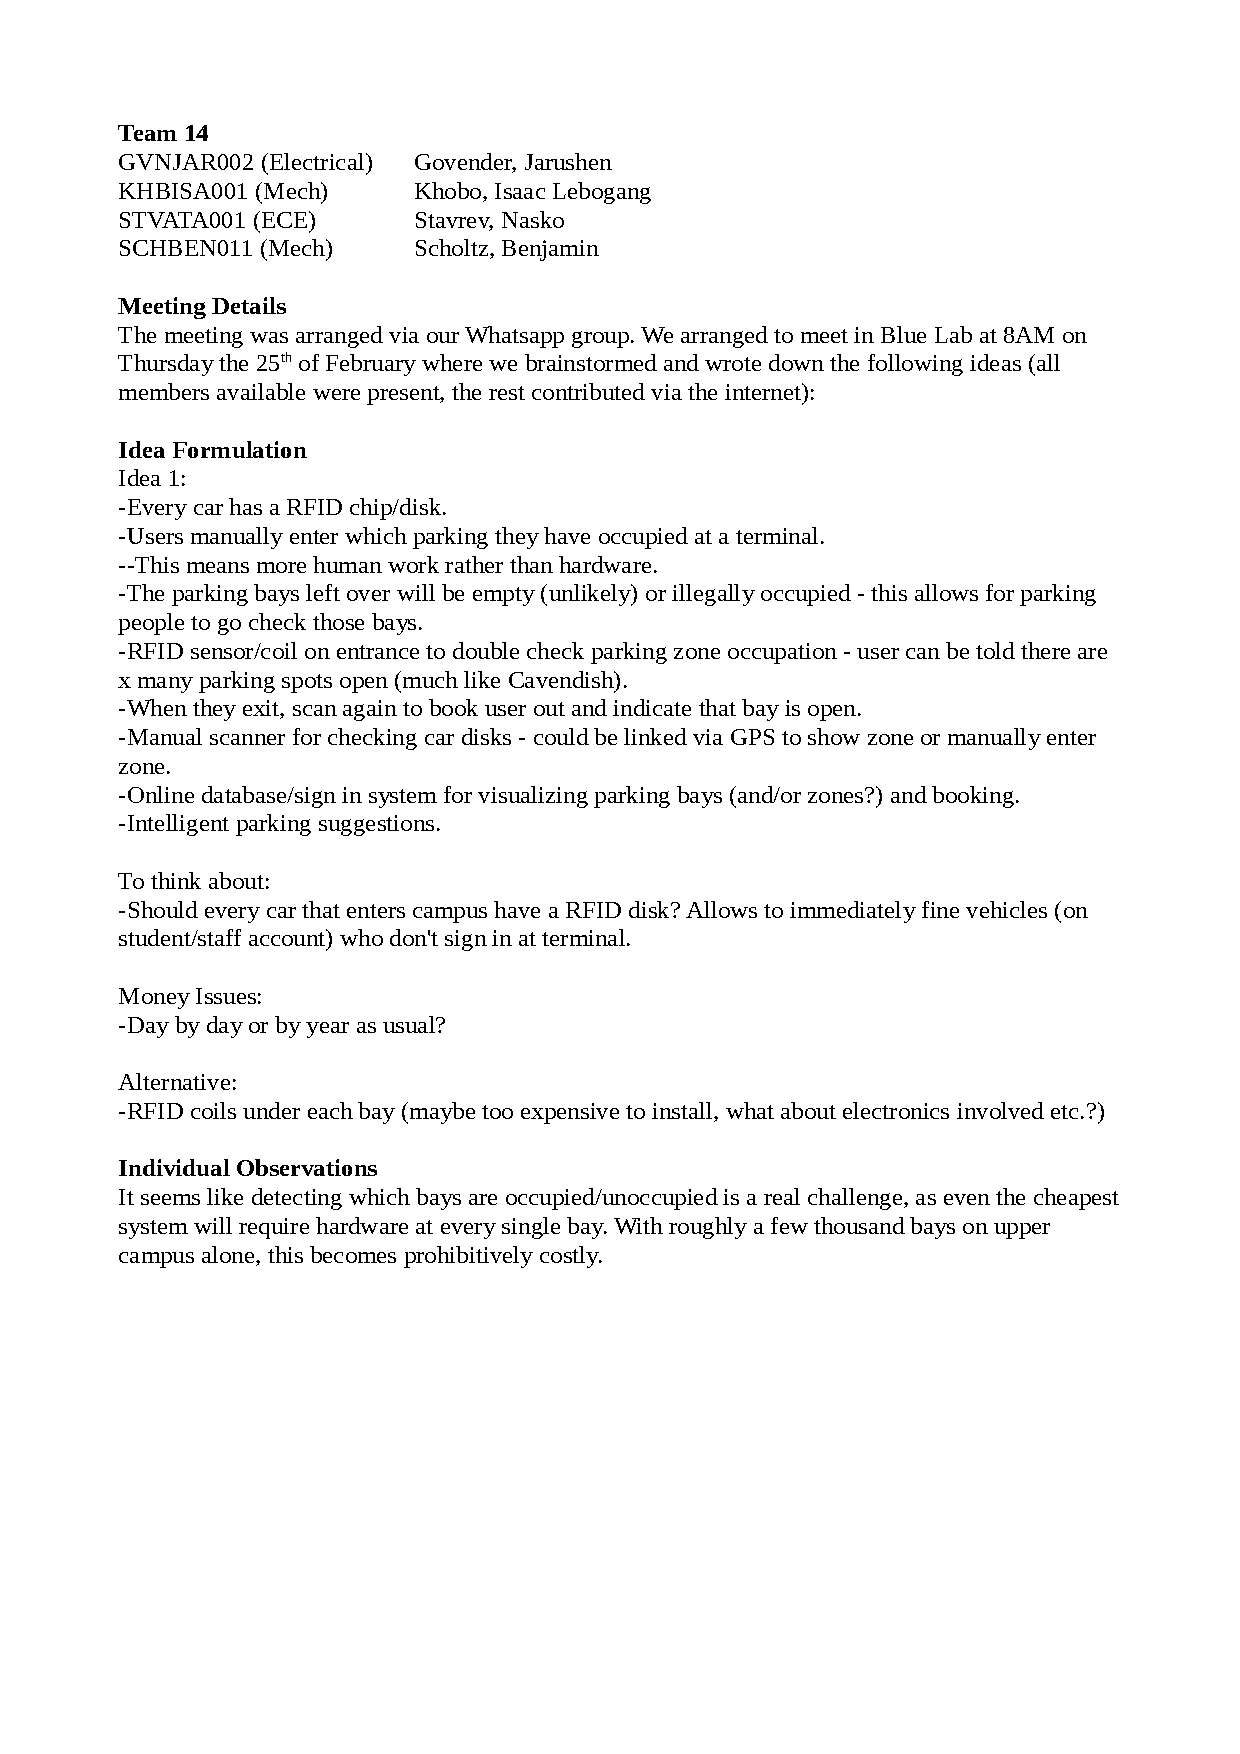
\includegraphics[scale=0.9]{meeting/report1-nasko.pdf}

\newpage
\subsection*{Progress Report 1: KHBISA001}
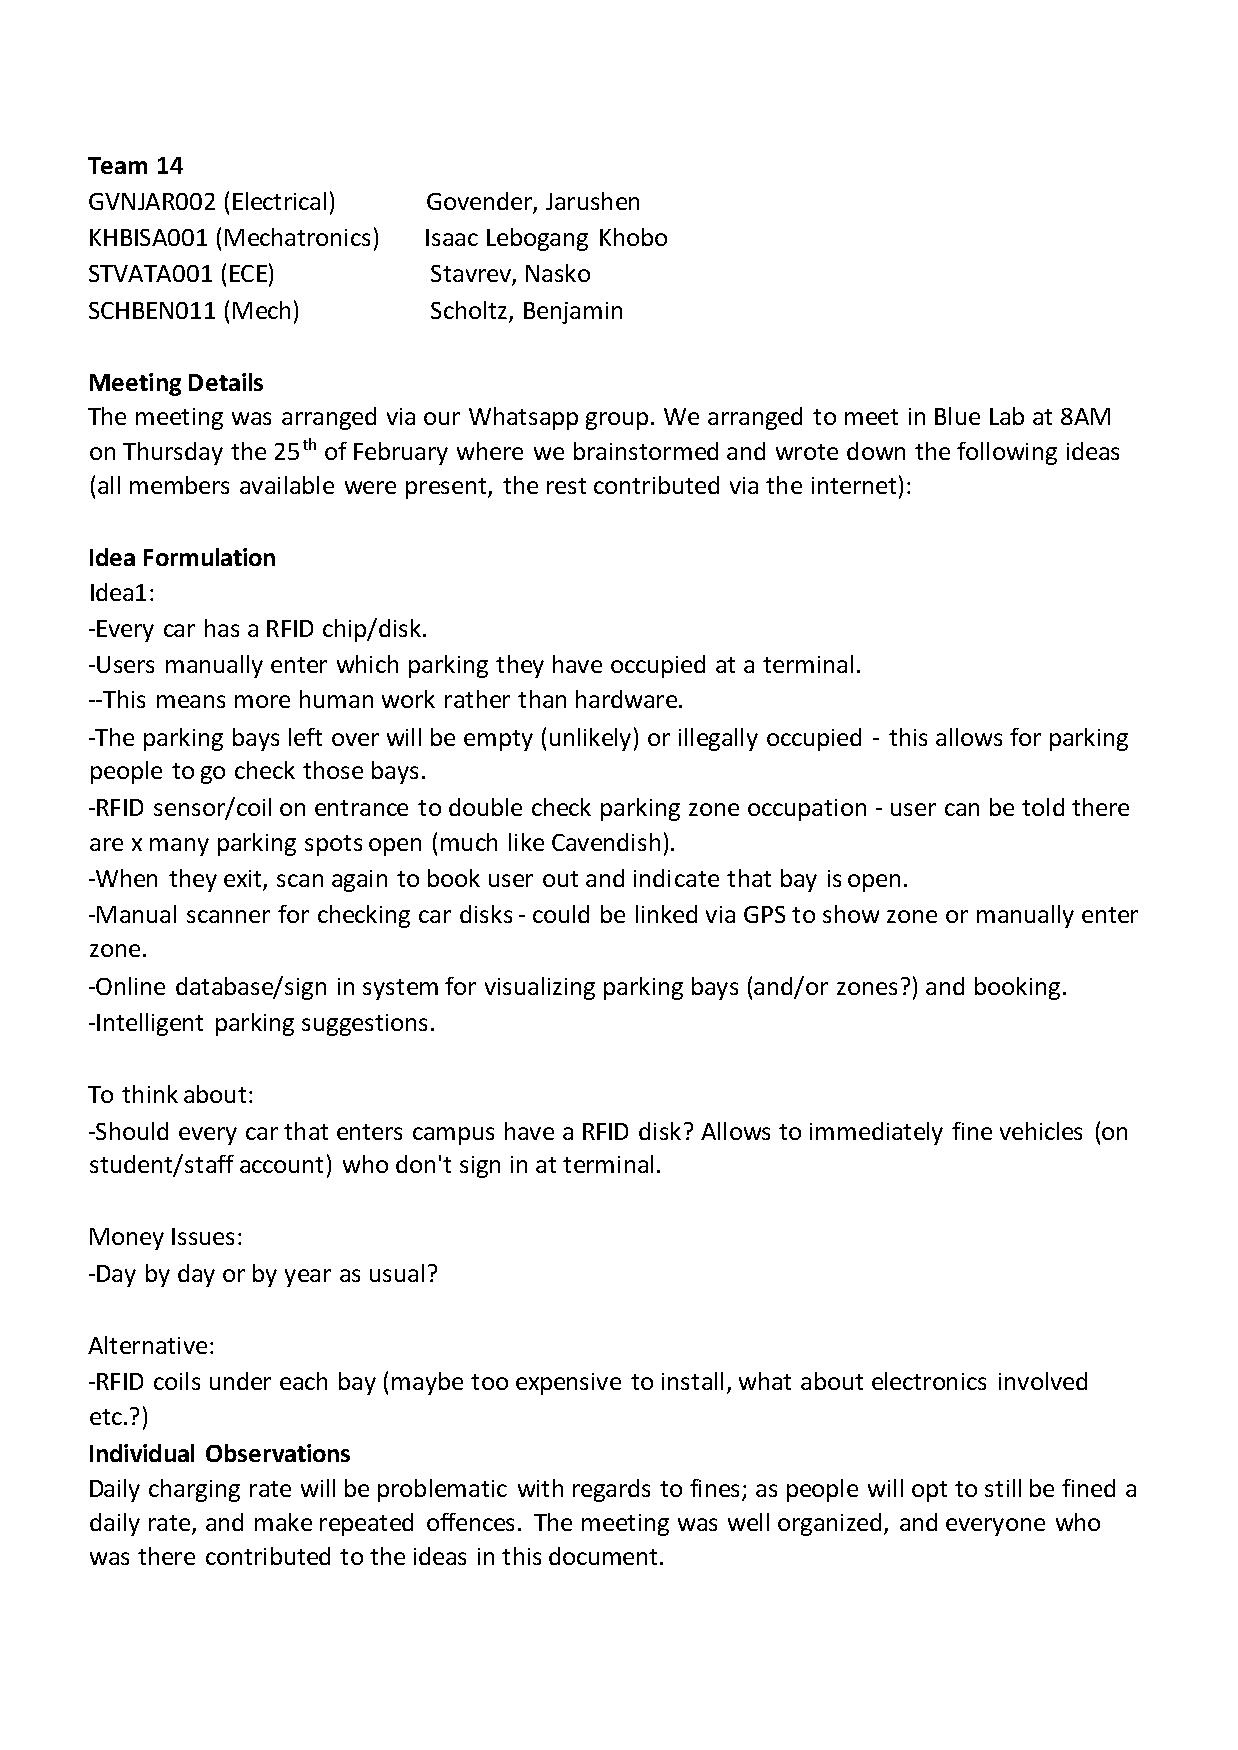
\includegraphics[scale=0.9]{meeting/report1-isaac.pdf}

\newpage
\subsection*{Progress Report 1: GVNJAR002}
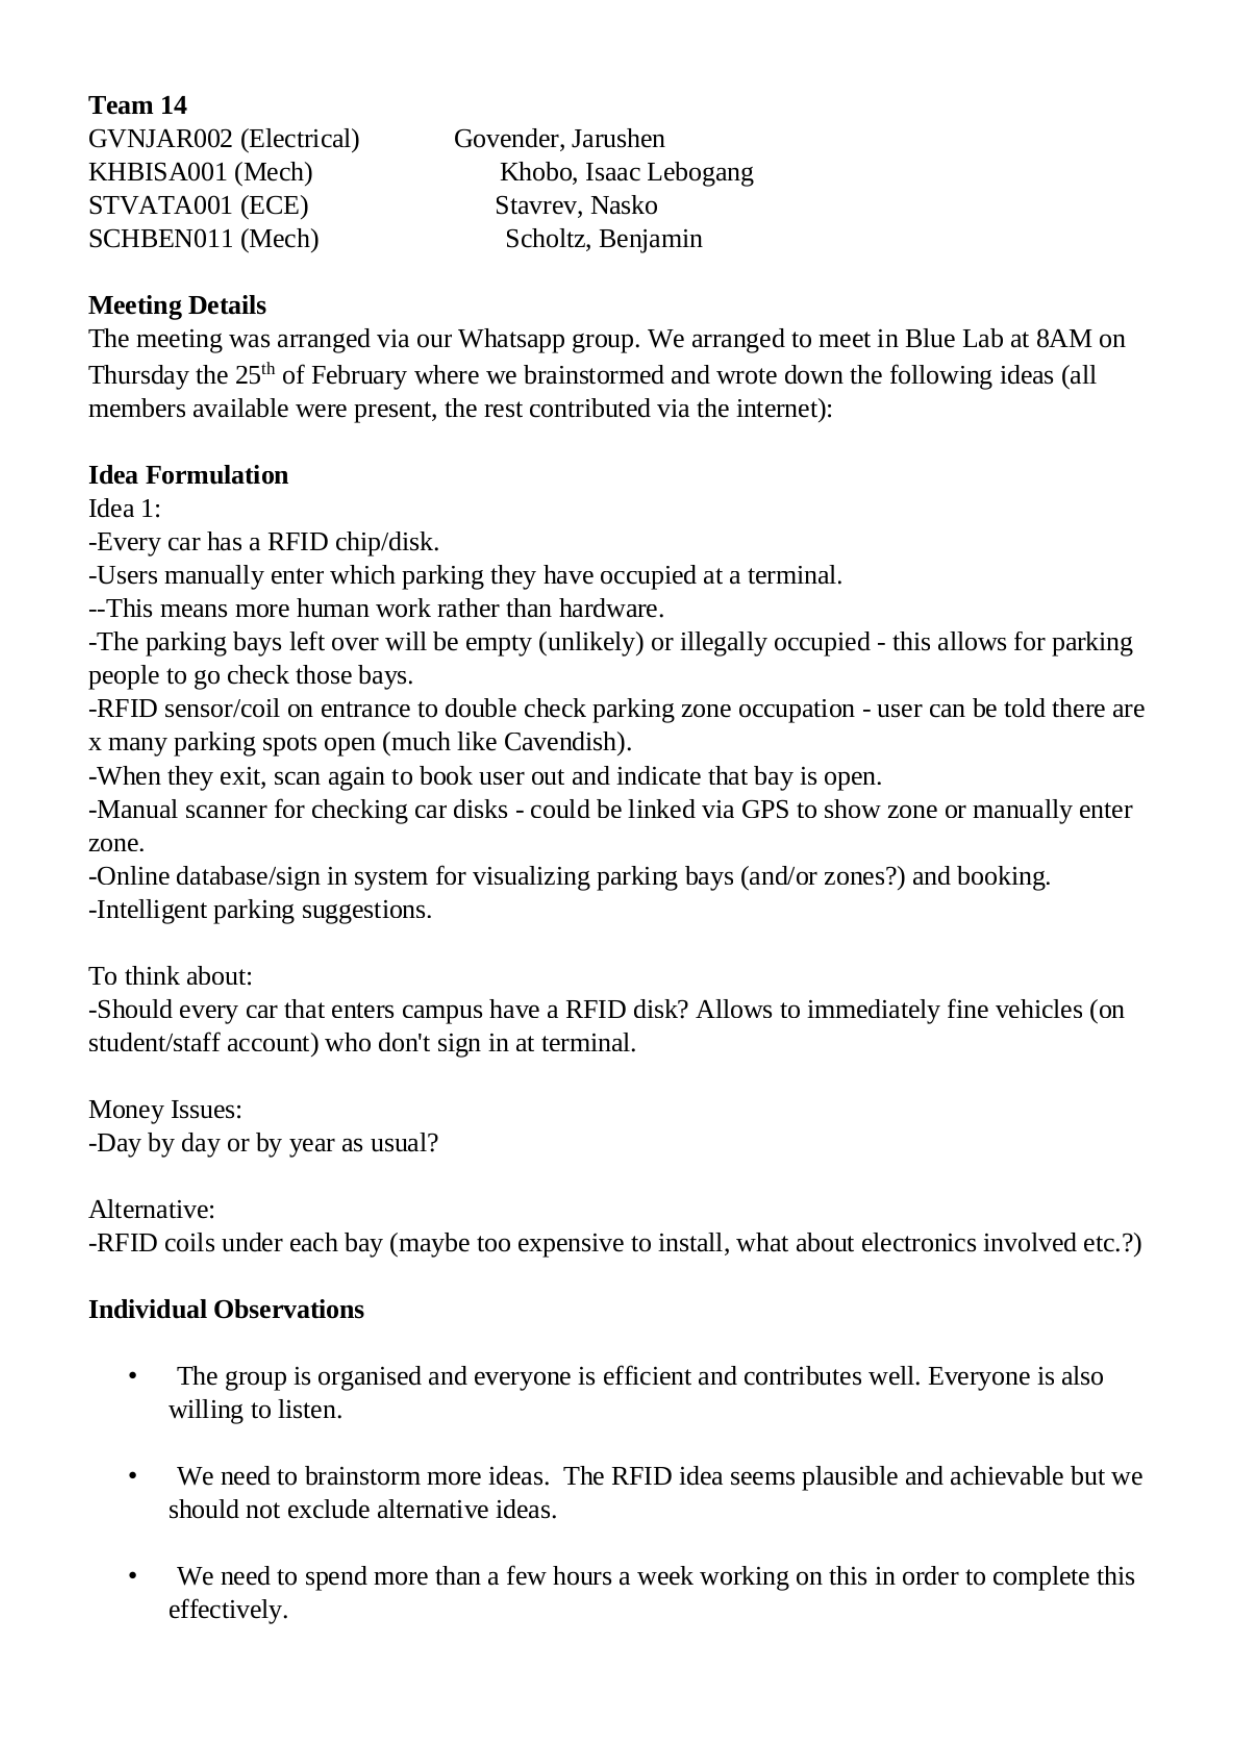
\includegraphics[scale=0.8]{meeting/report1-jarushen.pdf}

\newpage
\subsection*{Progress Report 2}
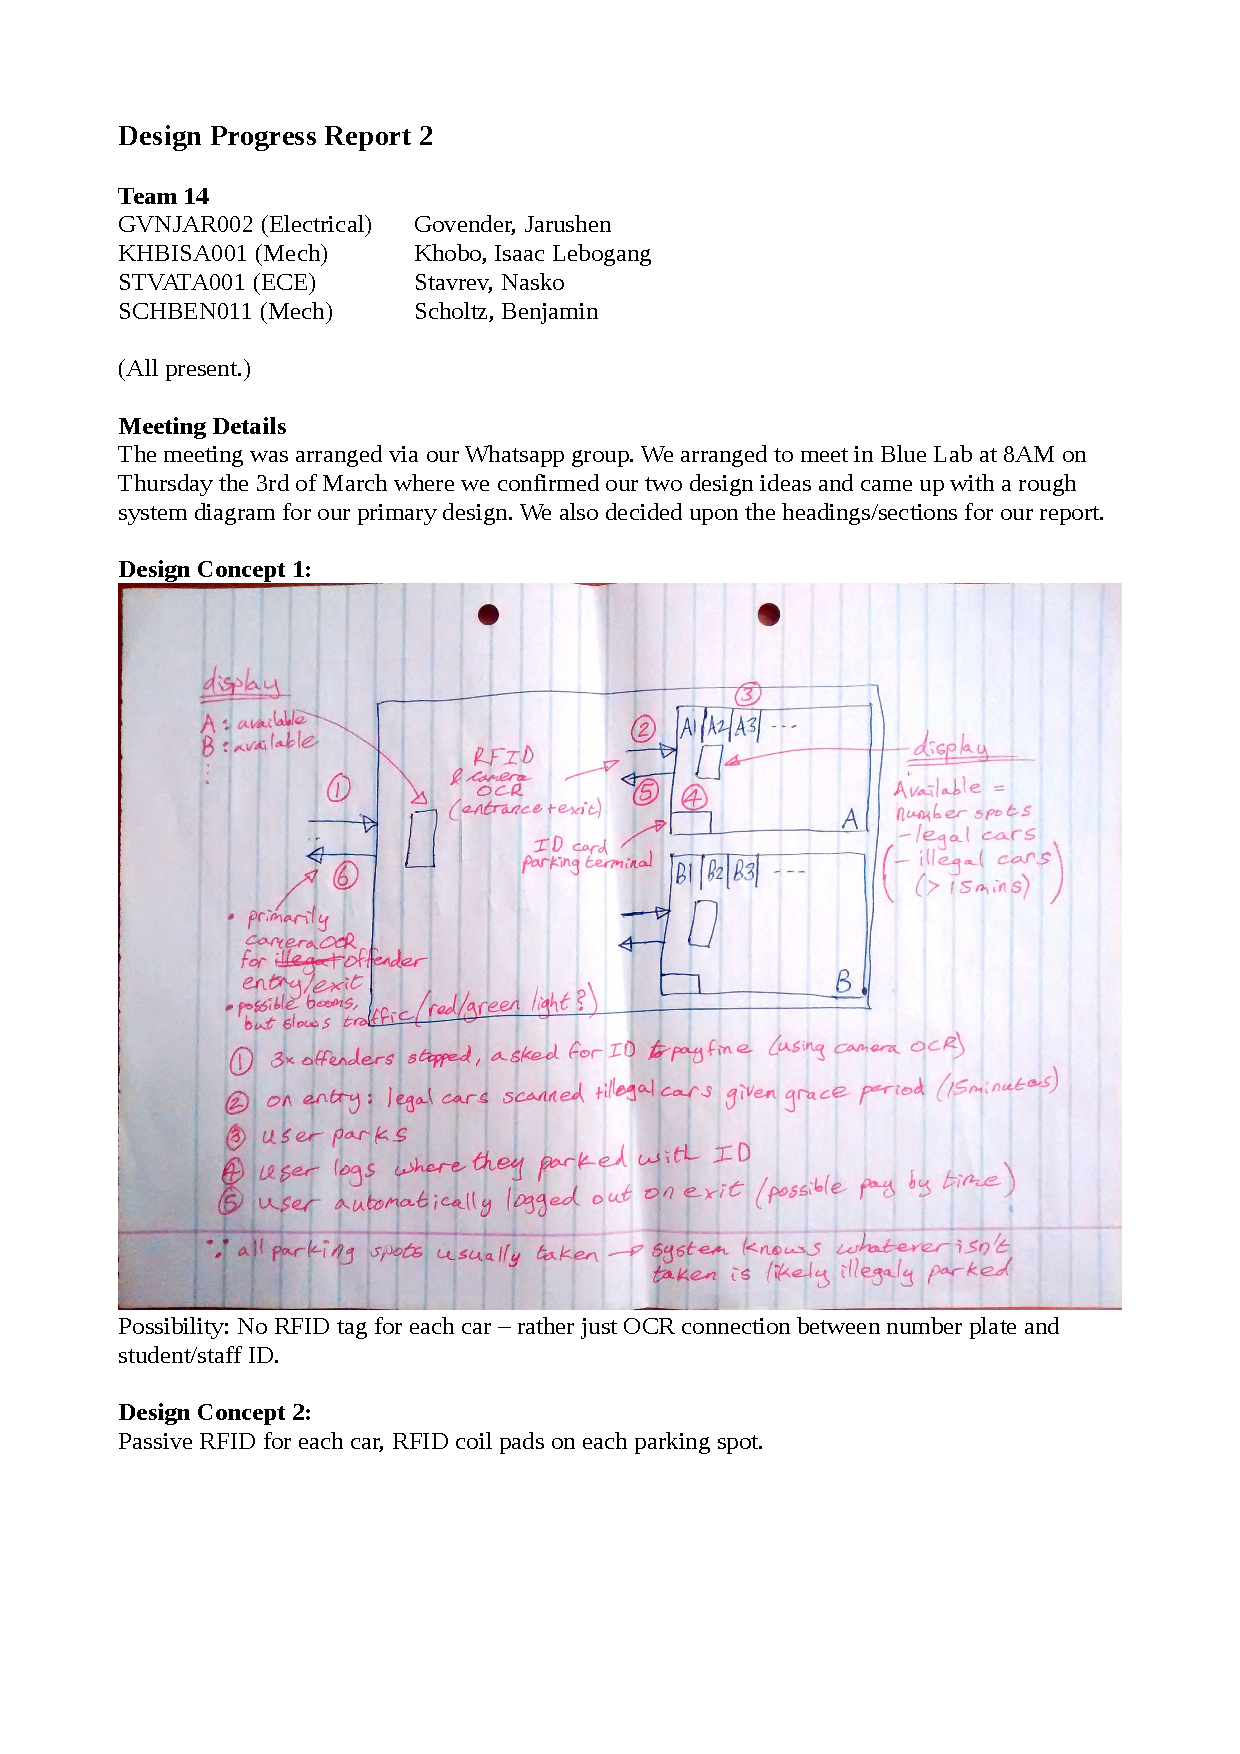
\includegraphics[scale=0.9]{meeting/report2-ben.pdf}
\includegraphics[page=2,scale=0.9]{meeting/report2-ben.pdf}

\newpage
\subsection*{Progress Report 3}
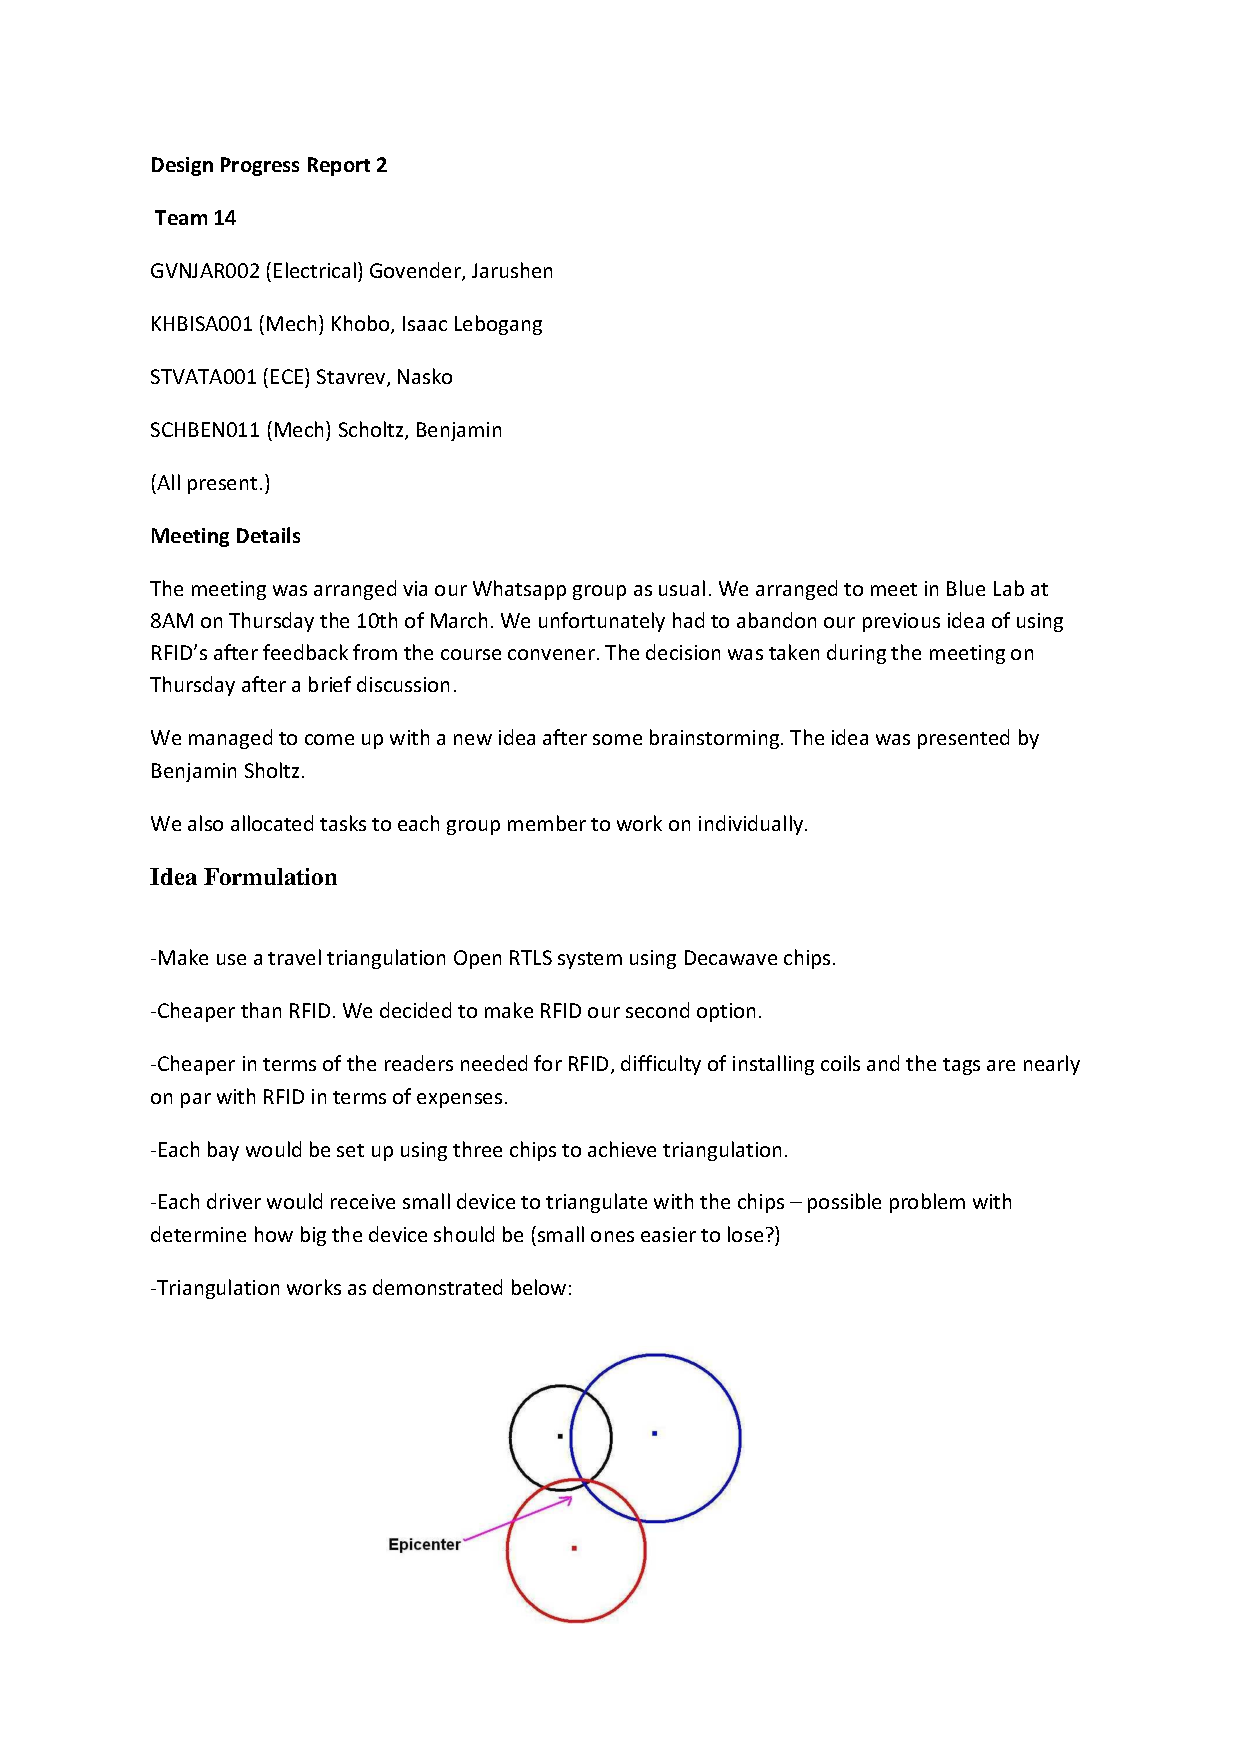
\includegraphics[scale=0.85]{meeting/report3-jarushen.pdf}\\
\includegraphics[page=2,scale=0.9]{meeting/report3-jarushen.pdf}
\includegraphics[page=3,scale=0.9]{meeting/report3-jarushen.pdf}

\newpage
\subsection*{Progress Report 4}
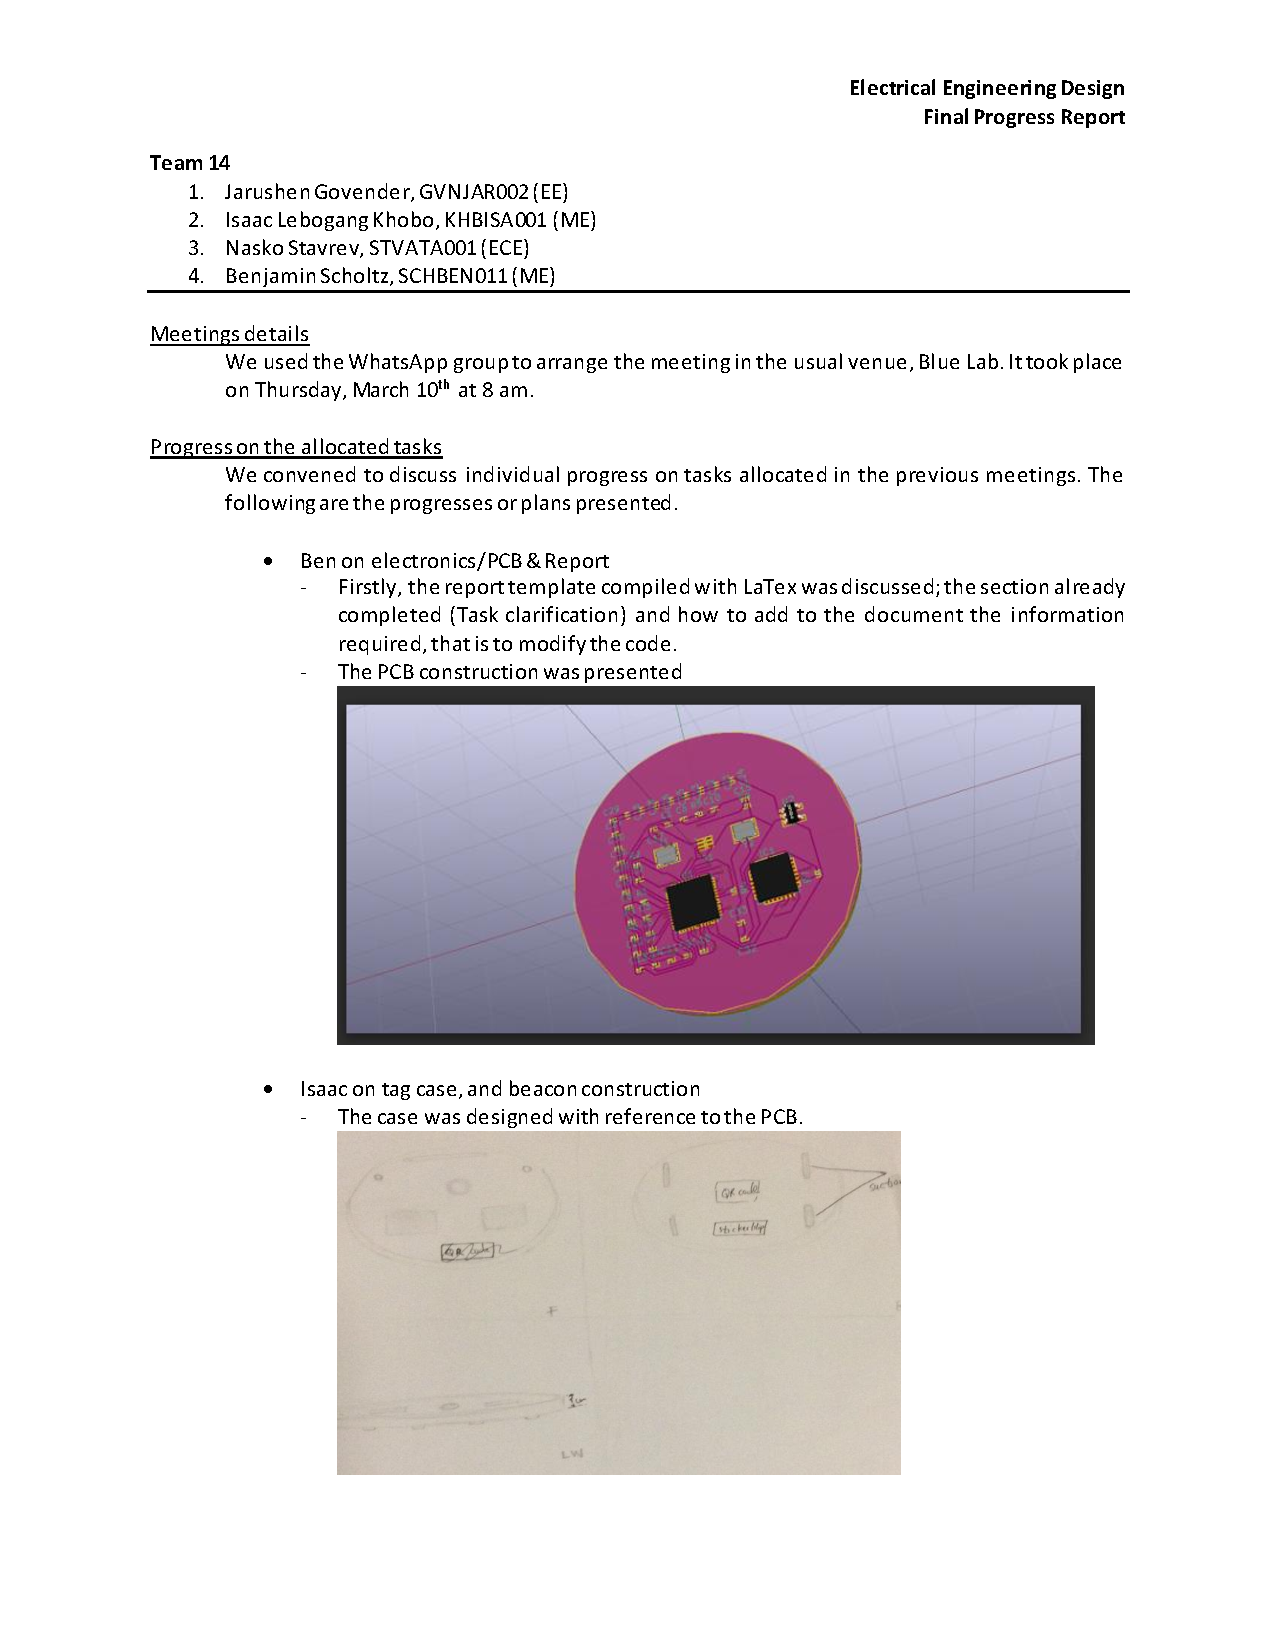
\includegraphics[scale=0.9]{meeting/report4-isaac.pdf}
\includegraphics[page=2,scale=0.9]{meeting/report4-isaac.pdf}
\includegraphics[page=3,scale=0.9]{meeting/report4-isaac.pdf}


\newpage
\vspace*{\fill}
\begin{center}
\subsection*{Appendix C: Tag Schematic Diagram}
\end{center}
\vspace*{\fill}
\addcontentsline{toc}{section}{Appendix C: Tag Schematic Diagram}
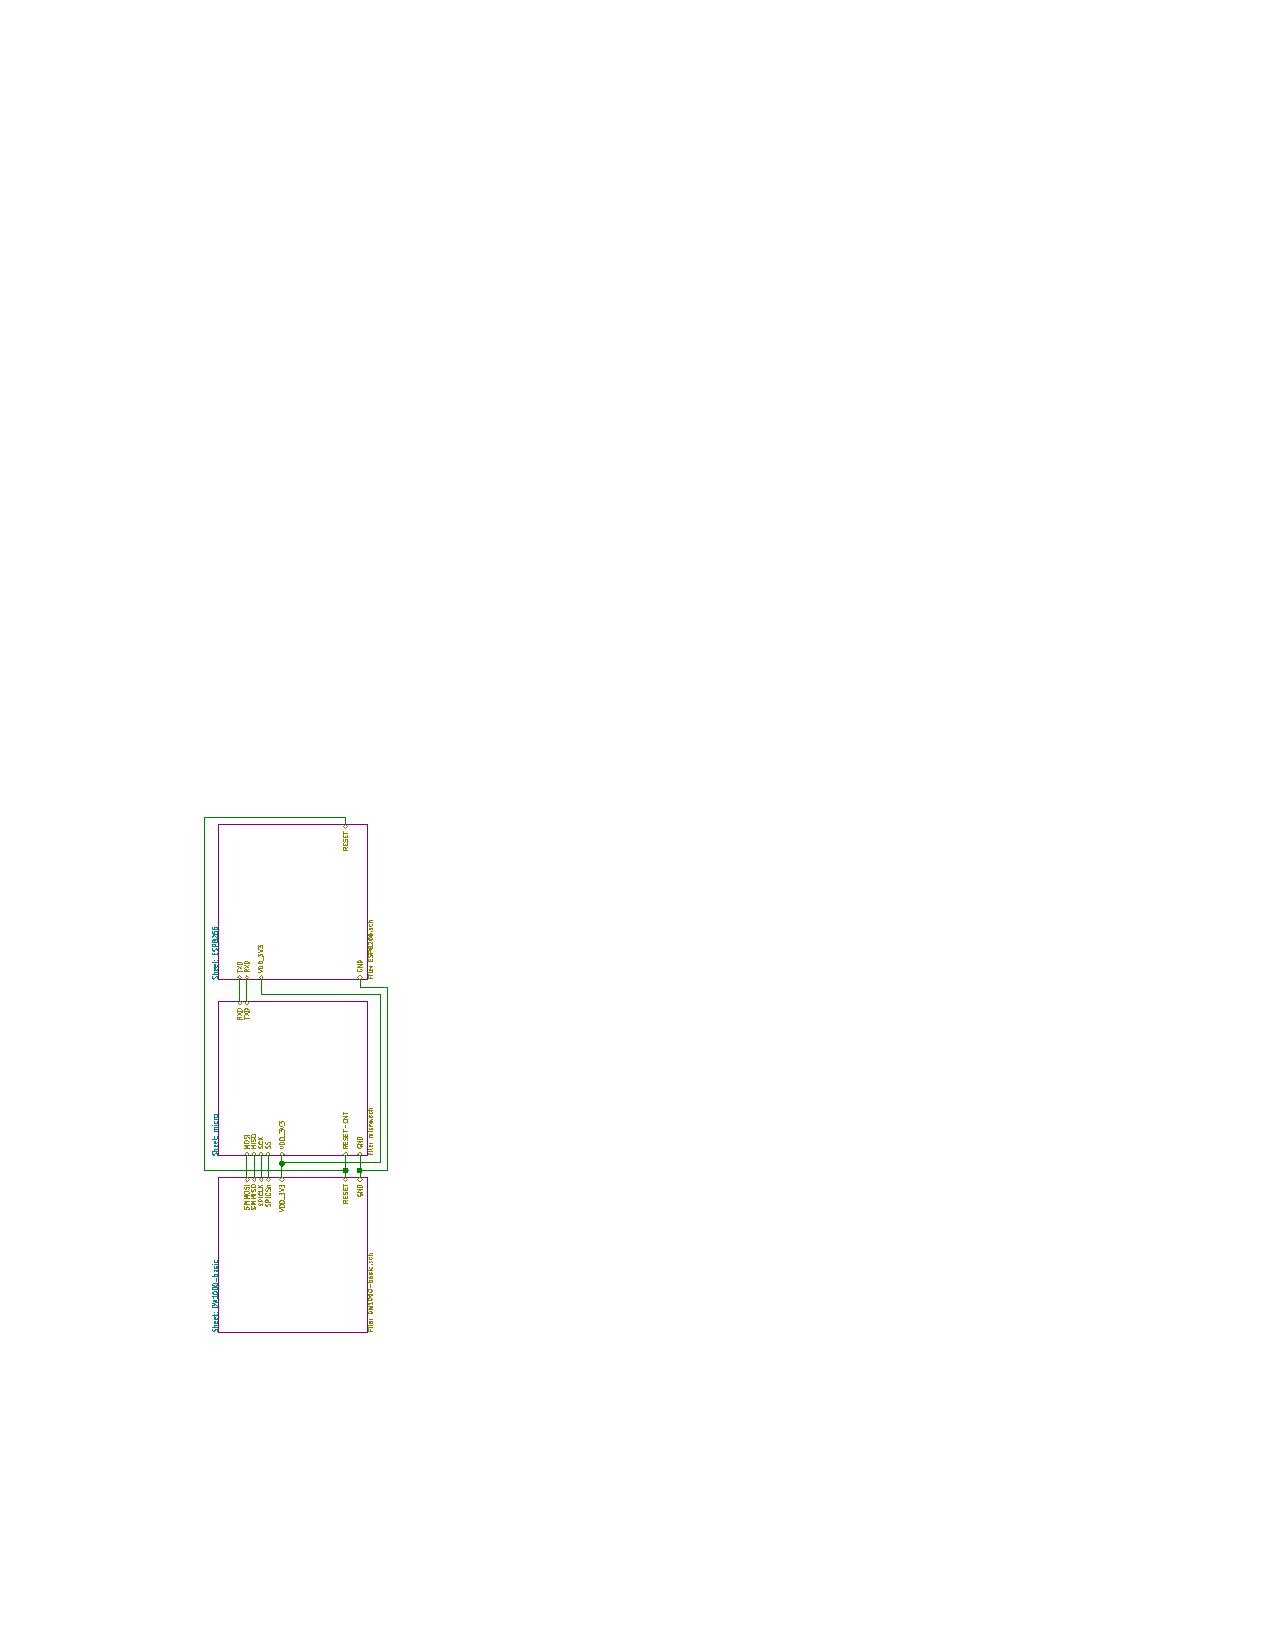
\includepdf[pages=-]{data/parking-system2.pdf}

\newpage
\vspace*{\fill}
\begin{center}
\subsection*{Appendix D: Tag PCB Layout}
\end{center}
\vspace*{\fill}
\addcontentsline{toc}{section}{Appendix D: Tag PCB Layout}
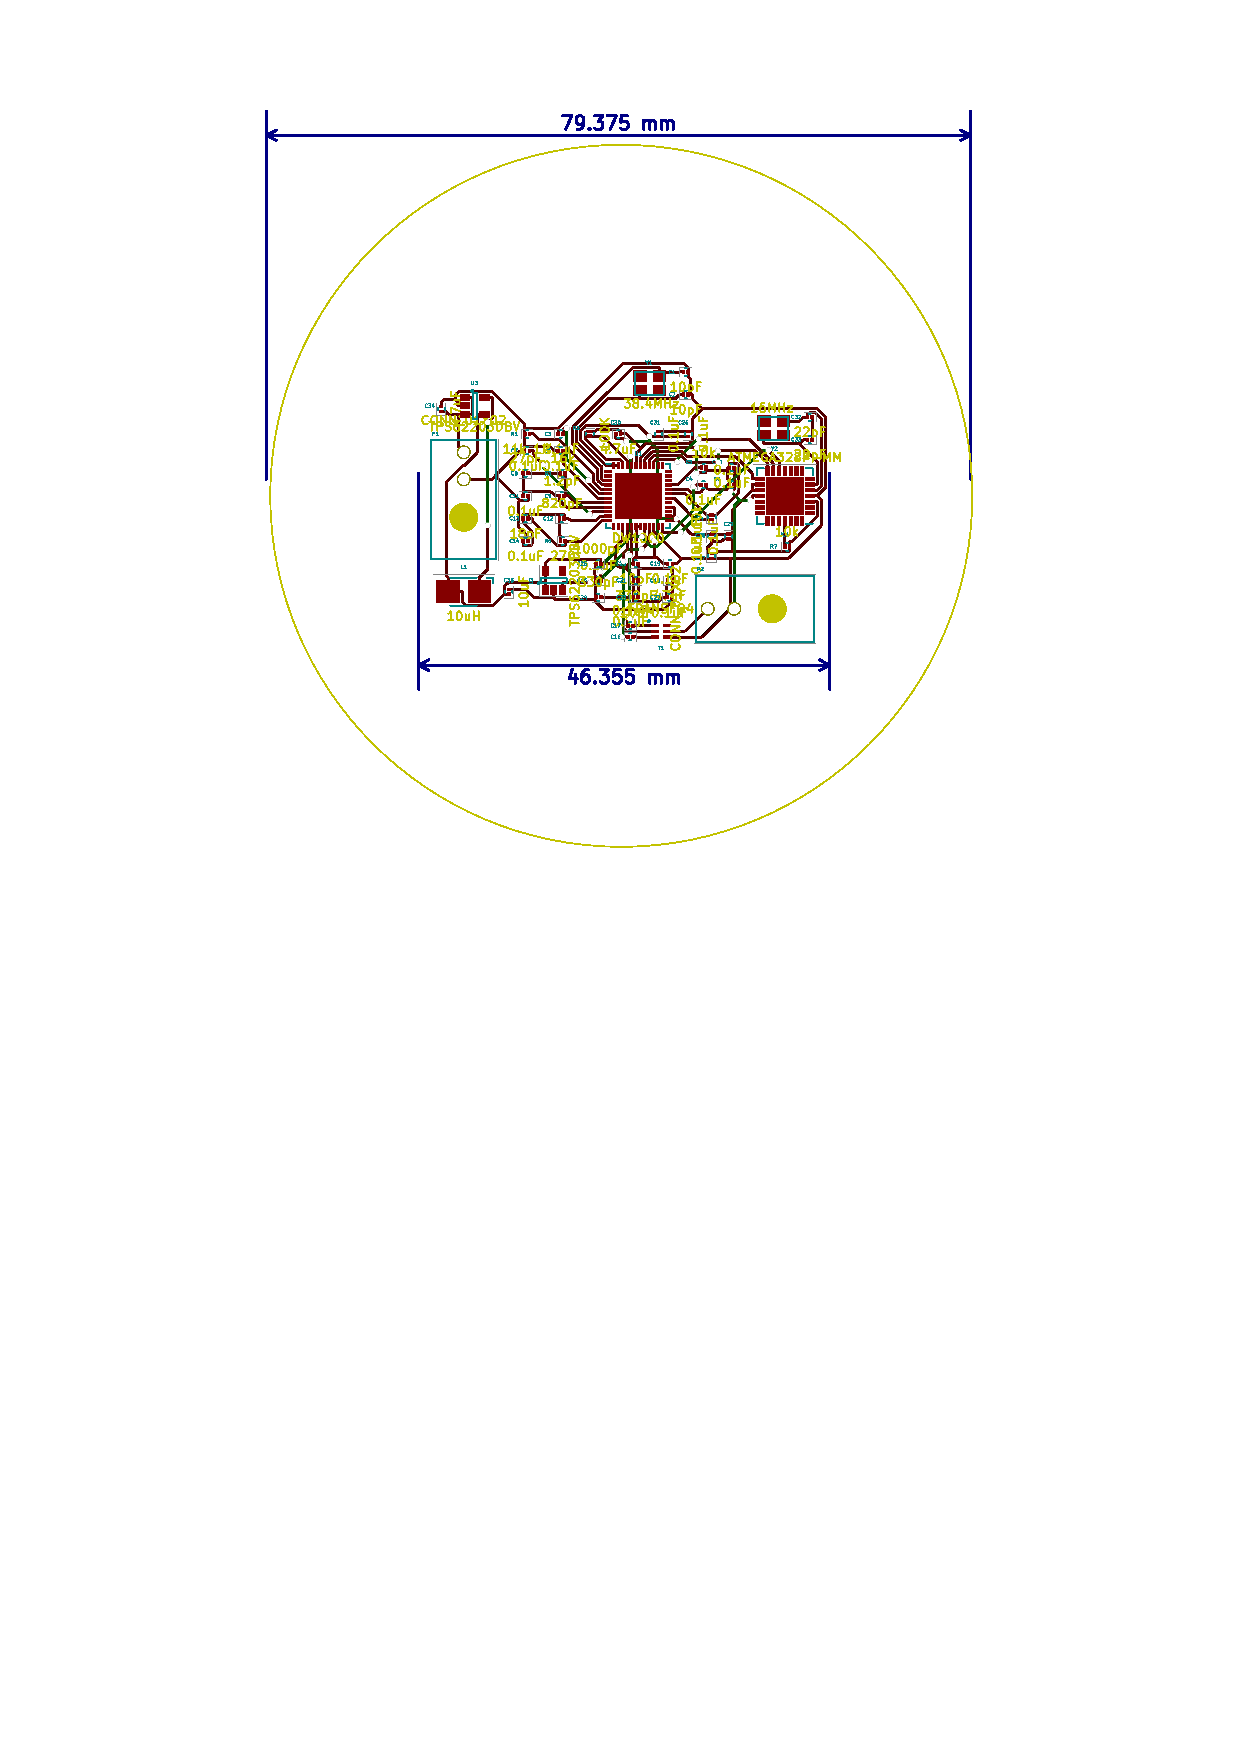
\includepdf[pages=-]{data/pcb-layout.pdf}

\newpage
\vspace*{\fill}
\begin{center}
\subsection*{Appendix E: Beacon PCB Layout}
\end{center}
\vspace*{\fill}
\addcontentsline{toc}{section}{Appendix E: Beacon PCB Layout}
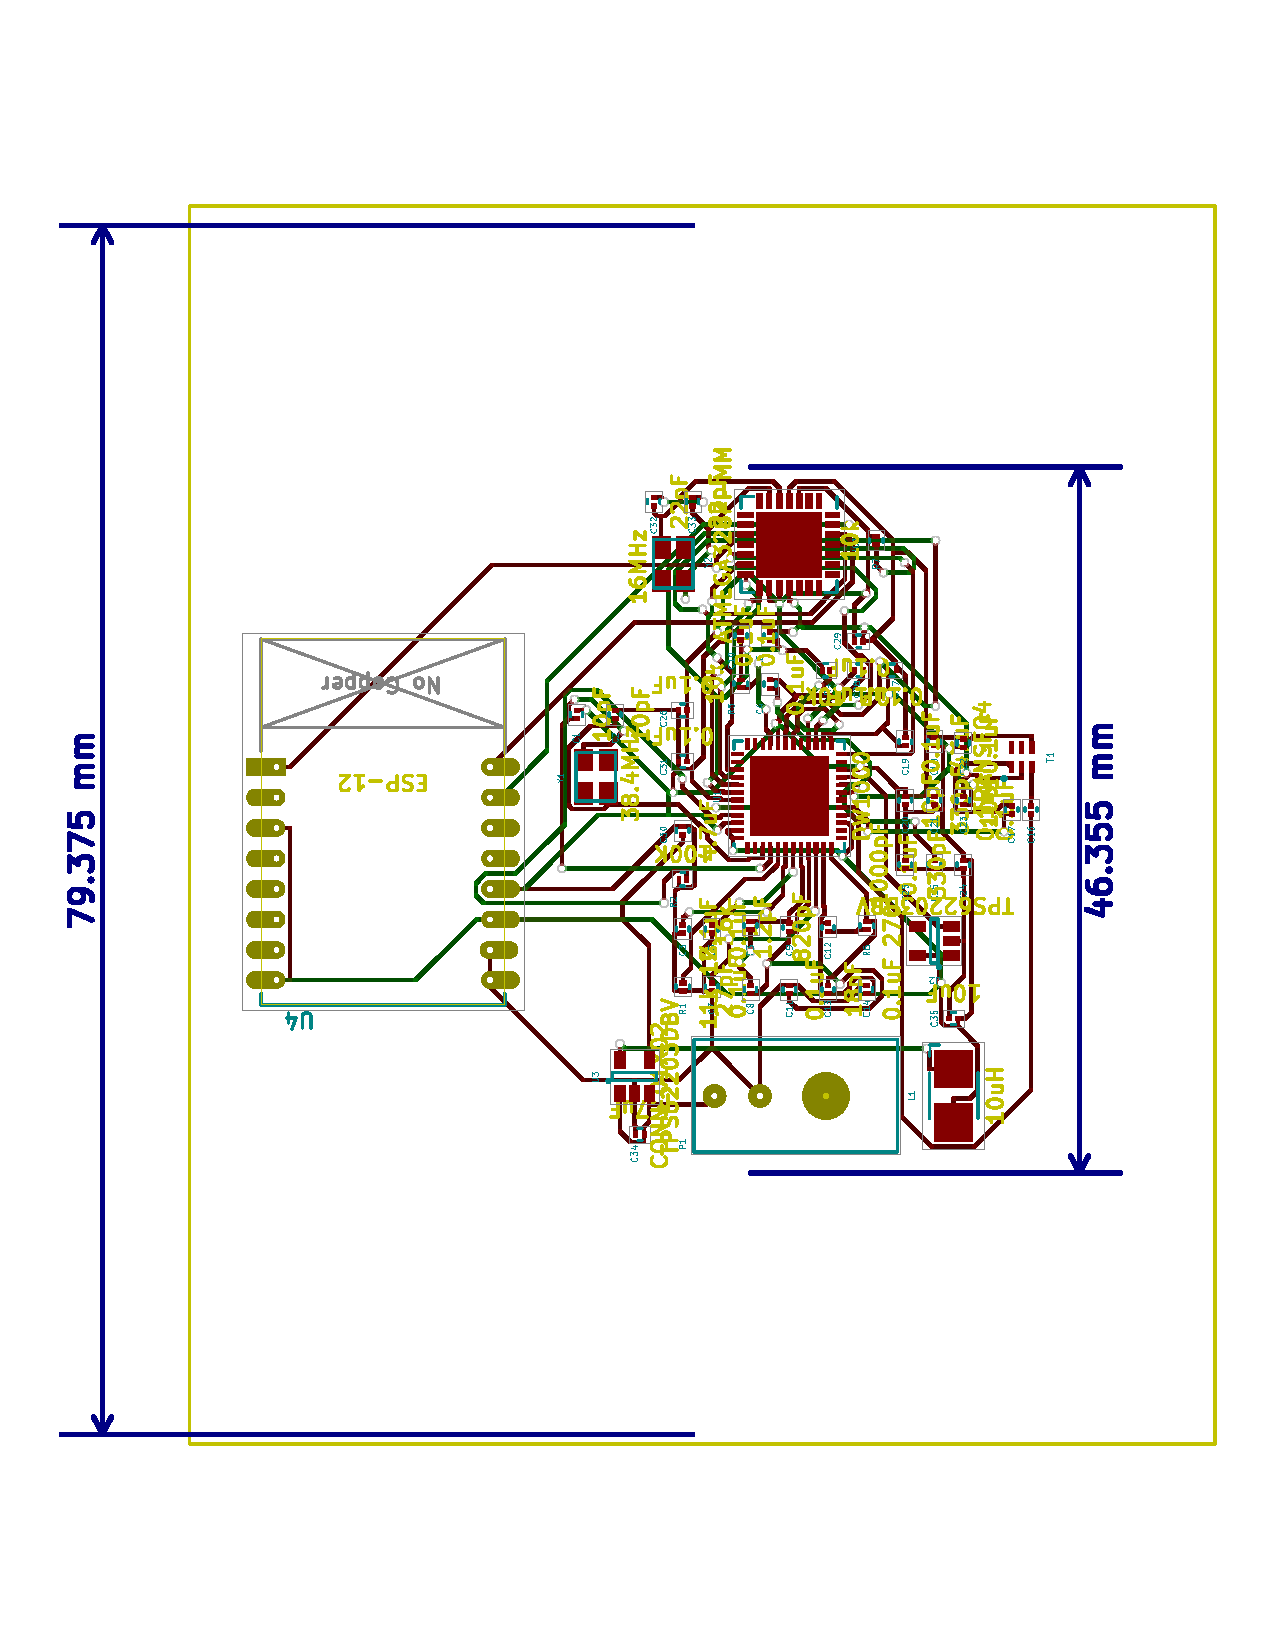
\includepdf[pages=-]{data/pcb-layout-ESP.pdf}

\newpage
\vspace*{\fill}
\begin{center}
\subsection*{Appendix F: Tag Bill of Materials and Unit Cost}
\end{center}
\vspace*{\fill}
\addcontentsline{toc}{section}{Appendix F: Tag Bill of Materials and Unit Cost}

\begin{landscape}
\begin{table}[]
\centering
\tiny
\caption{Tag Bill of Materials and Unit Cost Analysis}
\label{bom}
\begin{tabular}{llllllll}
\textbf{Ref}   & \textbf{Type} & \textbf{Value}             & \textbf{Footprint}              & \textbf{Part No. (Mouser default)}   & \textbf{Cost (US\$)} & \textbf{Outlay} & \textbf{Cost Outlay} \\
C4             & Capacitor     & 0.1uF                      & Capacitors\_SMD:C\_0201         & 81-GRM033R60J104KE19                 & 0.005                & 15000           & 75                   \\
C6             & Capacitor     & 0.1uF                      & Capacitors\_SMD:C\_0201         & 81-GRM033R60J104KE19                 & 0.005                & 15000           & 75                   \\
R2             & Resistor      & 100K                       & Resistors\_SMD:R\_0201          & 660-RK73H1HTTC1003F                  & 0.01                 & 15000           & 150                  \\
C31            & Capacitor     & 0.1uF                      & Capacitors\_SMD:C\_0201         & 81-GRM033R60J104KE19                 & 0.005                & 15000           & 75                   \\
C30            & Capacitor     & 4.7uF                      & Capacitors\_SMD:C\_0201         & 963-JMK063BJ474KP-F                  & 0.041                & 15000           & 615                  \\
C29            & Capacitor     & 0.1uF                      & Capacitors\_SMD:C\_0201         & 81-GRM033R60J104KE19                 & 0.005                & 15000           & 75                   \\
C28            & Capacitor     & 0.1uF                      & Capacitors\_SMD:C\_0201         & 81-GRM033R60J104KE19                 & 0.005                & 15000           & 75                   \\
C27            & Capacitor     & 0.1uF                      & Capacitors\_SMD:C\_0201         & 81-GRM033R60J104KE19                 & 0.005                & 15000           & 75                   \\
C26            & Capacitor     & 0.1uF                      & Capacitors\_SMD:C\_0201         & 81-GRM033R60J104KE19                 & 0.005                & 15000           & 75                   \\
C25            & Capacitor     & 1000pF                     & Capacitors\_SMD:C\_0201         & 81-GRM033R71E102KA1D                 & 0.004                & 15000           & 60                   \\
C24            & Capacitor     & 330pF                      & Capacitors\_SMD:C\_0201         & 81-GRM033R71E331KA1D                 & 0.004                & 15000           & 60                   \\
C23            & Capacitor     & 10pF                       & Capacitors\_SMD:C\_0201         & 81-GRM0335C1E100JA1D                 & 0.003                & 15000           & 45                   \\
C22            & Capacitor     & 0.1uF                      & Capacitors\_SMD:C\_0201         & 81-GRM033R60J104KE19                 & 0.005                & 15000           & 75                   \\
C21            & Capacitor     & 330pF                      & Capacitors\_SMD:C\_0201         & 81-GRM033R71E331KA1D                 & 0.004                & 15000           & 60                   \\
C20            & Capacitor     & 10pF                       & Capacitors\_SMD:C\_0201         & 81-GRM0335C1E100JA1D                 & 0.003                & 15000           & 45                   \\
C19            & Capacitor     & 0.1uF                      & Capacitors\_SMD:C\_0201         & 81-GRM033R60J104KE19                 & 0.005                & 15000           & 75                   \\
C18            & Capacitor     & 47uF                       & Capacitors\_SMD:C\_0201         & 581-TPSC476K016R0350                 & 0.206                & 15000           & 3090                 \\
C15            & Capacitor     & 0.1uF                      & Capacitors\_SMD:C\_0201         & 81-GRM033R60J104KE19                 & 0.005                & 15000           & 75                   \\
C17            & Capacitor     & 0.1uF                      & Capacitors\_SMD:C\_0201         & 81-GRM033R60J104KE19                 & 0.005                & 15000           & 75                   \\
C16            & Capacitor     & 0.1uF                      & Capacitors\_SMD:C\_0201         & 81-GRM033R60J104KE19                 & 0.005                & 15000           & 75                   \\
T1             & Transformer   & TRANSFO4                   & footprints:HHM1595A1            & 810-HHM1595A1                        & 0.362                & 15000           & 5430                 \\
C14            & Capacitor     & 0.1uF                      & Capacitors\_SMD:C\_0201         & 81-GRM033R60J104KE19                 & 0.005                & 15000           & 75                   \\
R6             & Resistor      & 270                        & Resistors\_SMD:R\_0201          & 667-ERJ-1GNF2700C                    & 0.005                & 15000           & 75                   \\
C12            & Capacitor     & 820pF                      & Capacitors\_SMD:C\_0201         & 81-GRM033R71E821KA1D                 & 0.004                & 15000           & 60                   \\
C13            & Capacitor     & 18pF                       & Capacitors\_SMD:C\_0201         & 581-02013A180GAT2A                   & 0.099                & 15000           & 1485                 \\
C11            & Capacitor     & 0.1uF                      & Capacitors\_SMD:C\_0201         & 81-GRM033R60J104KE19                 & 0.005                & 15000           & 75                   \\
C9             & Capacitor     & 1.2pF                      & Capacitors\_SMD:C\_0201         & 810-C0603C0G1E1R2BTQ                 & 0.02                 & 15000           & 300                  \\
R3             & Resistor      & 16k                        & Resistors\_SMD:R\_0201          & 667-ERJ-1GEJ163C                     & 0.004                & 15000           & 60                   \\
C8             & Capacitor     & 27pF                       & Capacitors\_SMD:C\_0201         & 81-GRM0335C1E270JA1D                 & 0.004                & 15000           & 60                   \\
C7             & Capacitor     & 0.1uF                      & Capacitors\_SMD:C\_0201         & 81-GRM033R60J104KE19                 & 0.005                & 15000           & 75                   \\
R1             & Resistor      & 11k 1\%                    & Resistors\_SMD:R\_0201          & 71-CRCW020111K0FKED                  & 0.026                & 15000           & 390                  \\
C5             & Capacitor     & 0.1uF                      & Capacitors\_SMD:C\_0201         & 81-GRM033R60J104KE19                 & 0.005                & 15000           & 75                   \\
C3             & Capacitor     & 0.1uF                      & Capacitors\_SMD:C\_0201         & 81-GRM033R60J104KE19                 & 0.005                & 15000           & 75                   \\
R4             & Resistor      & 10k                        & Resistors\_SMD:R\_0201          & 603-RC0201FR-0710KL                  & 0.004                & 15000           & 60                   \\
R5             & Resistor      & 10k                        & Resistors\_SMD:R\_0201          & 603-RC0201FR-0710KL                  & 0.004                & 15000           & 60                   \\
C2             & Capacitor     & 10pF                       & Capacitors\_SMD:C\_0201         & 81-GRM0335C1E100JA1D                 & 0.003                & 15000           & 45                   \\
C1             & Capacitor     & 10pF                       & Capacitors\_SMD:C\_0201         & 81-GRM0335C1E100JA1D                 & 0.003                & 15000           & 45                   \\
Y1             & Crystal       & 38.4MHz                    & Crystals:FA238-TSX3225          & ABM10-165-38.400MHz-T3               & 0.667                & 15000           & 10005                \\
C10            & Capacitor     & 0.1uF                      & Capacitors\_SMD:C\_0201         & 81-GRM033R60J104KE19                 & 0.005                & 15000           & 75                   \\
U1             & Transciever   & DW1000                     & Housings\_DFN\_QFN:QFN-48       & 1479-1001-2-ND                       & 8.8726               & 15000           & 133089               \\
U2             & DC-DC         & TPS62203DBV                & SMD:SOT-23-5                    & 595-TPS62203DBVR                     & 0.542                & 15000           & 8130                 \\
U3             & DC-DC         & TPS62203DBV                & SMD:SOT-23-5                    & 595-TPS62203DBVR                     & 0.542                & 15000           & 8130                 \\
C34            & Capacitor     & 4.7uF                      & Capacitors\_SMD:C\_0201         & 963-JMK063BJ474KP-F                  & 0.041                & 15000           & 615                  \\
L1             & Inductor      & 10uH                       & Inductors:Inductor\_1212        & 81-LQH3NPN100MM0L                    & 0.132                & 15000           & 1980                 \\
C35            & Capacitor     & 10uF                       & Capacitors\_SMD:C\_0201         & 80-T491C106K016                      & 0.102                & 15000           & 1530                 \\
P1             & Connector     & CONN\_01X02                & Connectors\_Molex               & See note.                            & 0.5                  & 15000           & 7500                 \\
P2             & Antenna       & Antenna                    & PCB Chip Antenna                & 963-AH086M555003-T                   & 0.803                & 15000           & 12045                \\
IC1            & Micro.        & ATMEGA328P-MM              & DFN\_QFN:QFN-28                 & 556-ATMEGA328P-MMH                   & 1.89                 & 15000           & 28350                \\
R7             & Resistor      & 10k                        & Resistors\_SMD:R\_0201          & 603-RC0201FR-0710KL                  & 0.004                & 15000           & 60                   \\
Y2             & Crystal       & 16MHz                      & Crystals:crystal\_FA238-TSX3225 & 732-TX325-16F09Z-AC3                 & 0.278                & 15000           & 4170                 \\
C32            & Capacitor     & 22pF                       & Capacitors\_SMD:C\_0201         & 810-C0603C0G1H220J                   & 0.004                & 15000           & 60                   \\
C33            & Capacitor     & 22pF                       & Capacitors\_SMD:C\_0201         & 810-C0603C0G1H220J                   & 0.004                & 15000           & 60                   \\
               &               &                            &                                 & \textbf{Total Capital Outlay (ZAR):} &                      &                 & \textbf{3558254.88}  \\
               &               &                            &                                 & \textbf{Unit Cost (ZAR):}            &                      &                 & \textbf{237.216992}  \\
               &               &                            &                                 &                                      &                      &                 &                      \\
\textbf{Notes} &               &                            &                                 &                                      &                      &                 &                      \\
P1             & Connector     & Part No.: Diff. Footprint. &                                 &                                      &                      &                 &                      \\
C35            & Capacitor     & Footprint: 2412            &                                 &                                      &                      &                 &                      \\
U1             & Transciever   & Supplier: Digikey          &                                 &                                      &                      &                 &                     
\end{tabular}
\end{table}
\end{landscape}

\end{document}

%----------------------------------------------------------------------------


